% Generated by build_corner_treatment_figure_report.py -- do not edit by hand; rerun the script.
\documentclass[11pt]{article}
\usepackage[a4paper,margin=0.8in]{geometry}
\usepackage[T1]{fontenc}
\usepackage[utf8]{inputenc}
\usepackage[french]{babel}
\usepackage{amsmath,amssymb}
\usepackage{booktabs}
\usepackage{graphicx}
\usepackage{adjustbox}
\usepackage{float}
\usepackage{xcolor}
\usepackage{pdflscape}
\usepackage{url}
\urlstyle{tt}
\usepackage[colorlinks=true,allcolors=blue!55!black]{hyperref}
\title{Down-and-out put --- traitements du coin : figures}
\author{}
\date{2026-09-21}
\begin{document}
\maketitle
\tableofcontents
\clearpage
Recueil des figures et tables produites par les scripts d'agrégation, sans aucun recalcul : chaque légende indique ce qui est tracé ; les chemins des artefacts sources sont donnés en tête de section. Notation : $\Delta=K-B$, $V_{DOD}$ le prix du digital down-and-out, $\xi=\ln(s/B)/(\sigma\sqrt{2(T-t)})$, $\chi$ le cutoff de l'enrichissement, $N_{0.1}=\{|s-B|+(T-t)\le0.1\}$ la fenêtre de coin des métriques.

\section{Comparaison entre configurations (médianes sur les graines)}
Chaque point est une graine maîtresse, le losange plein la médiane. Les configurations de lissage excluent la fenêtre de coin $N_{0.1}$ de la collocation ; les traitements analytiques (soustraction, enrichissement) incluent le coin, ce que l'étiquette de l'axe rappelle. Source : \path{data/aggregate_terminal_function_comparison/20260921_corner_treatments_iters50000}.
\begin{figure}[H]
\centering
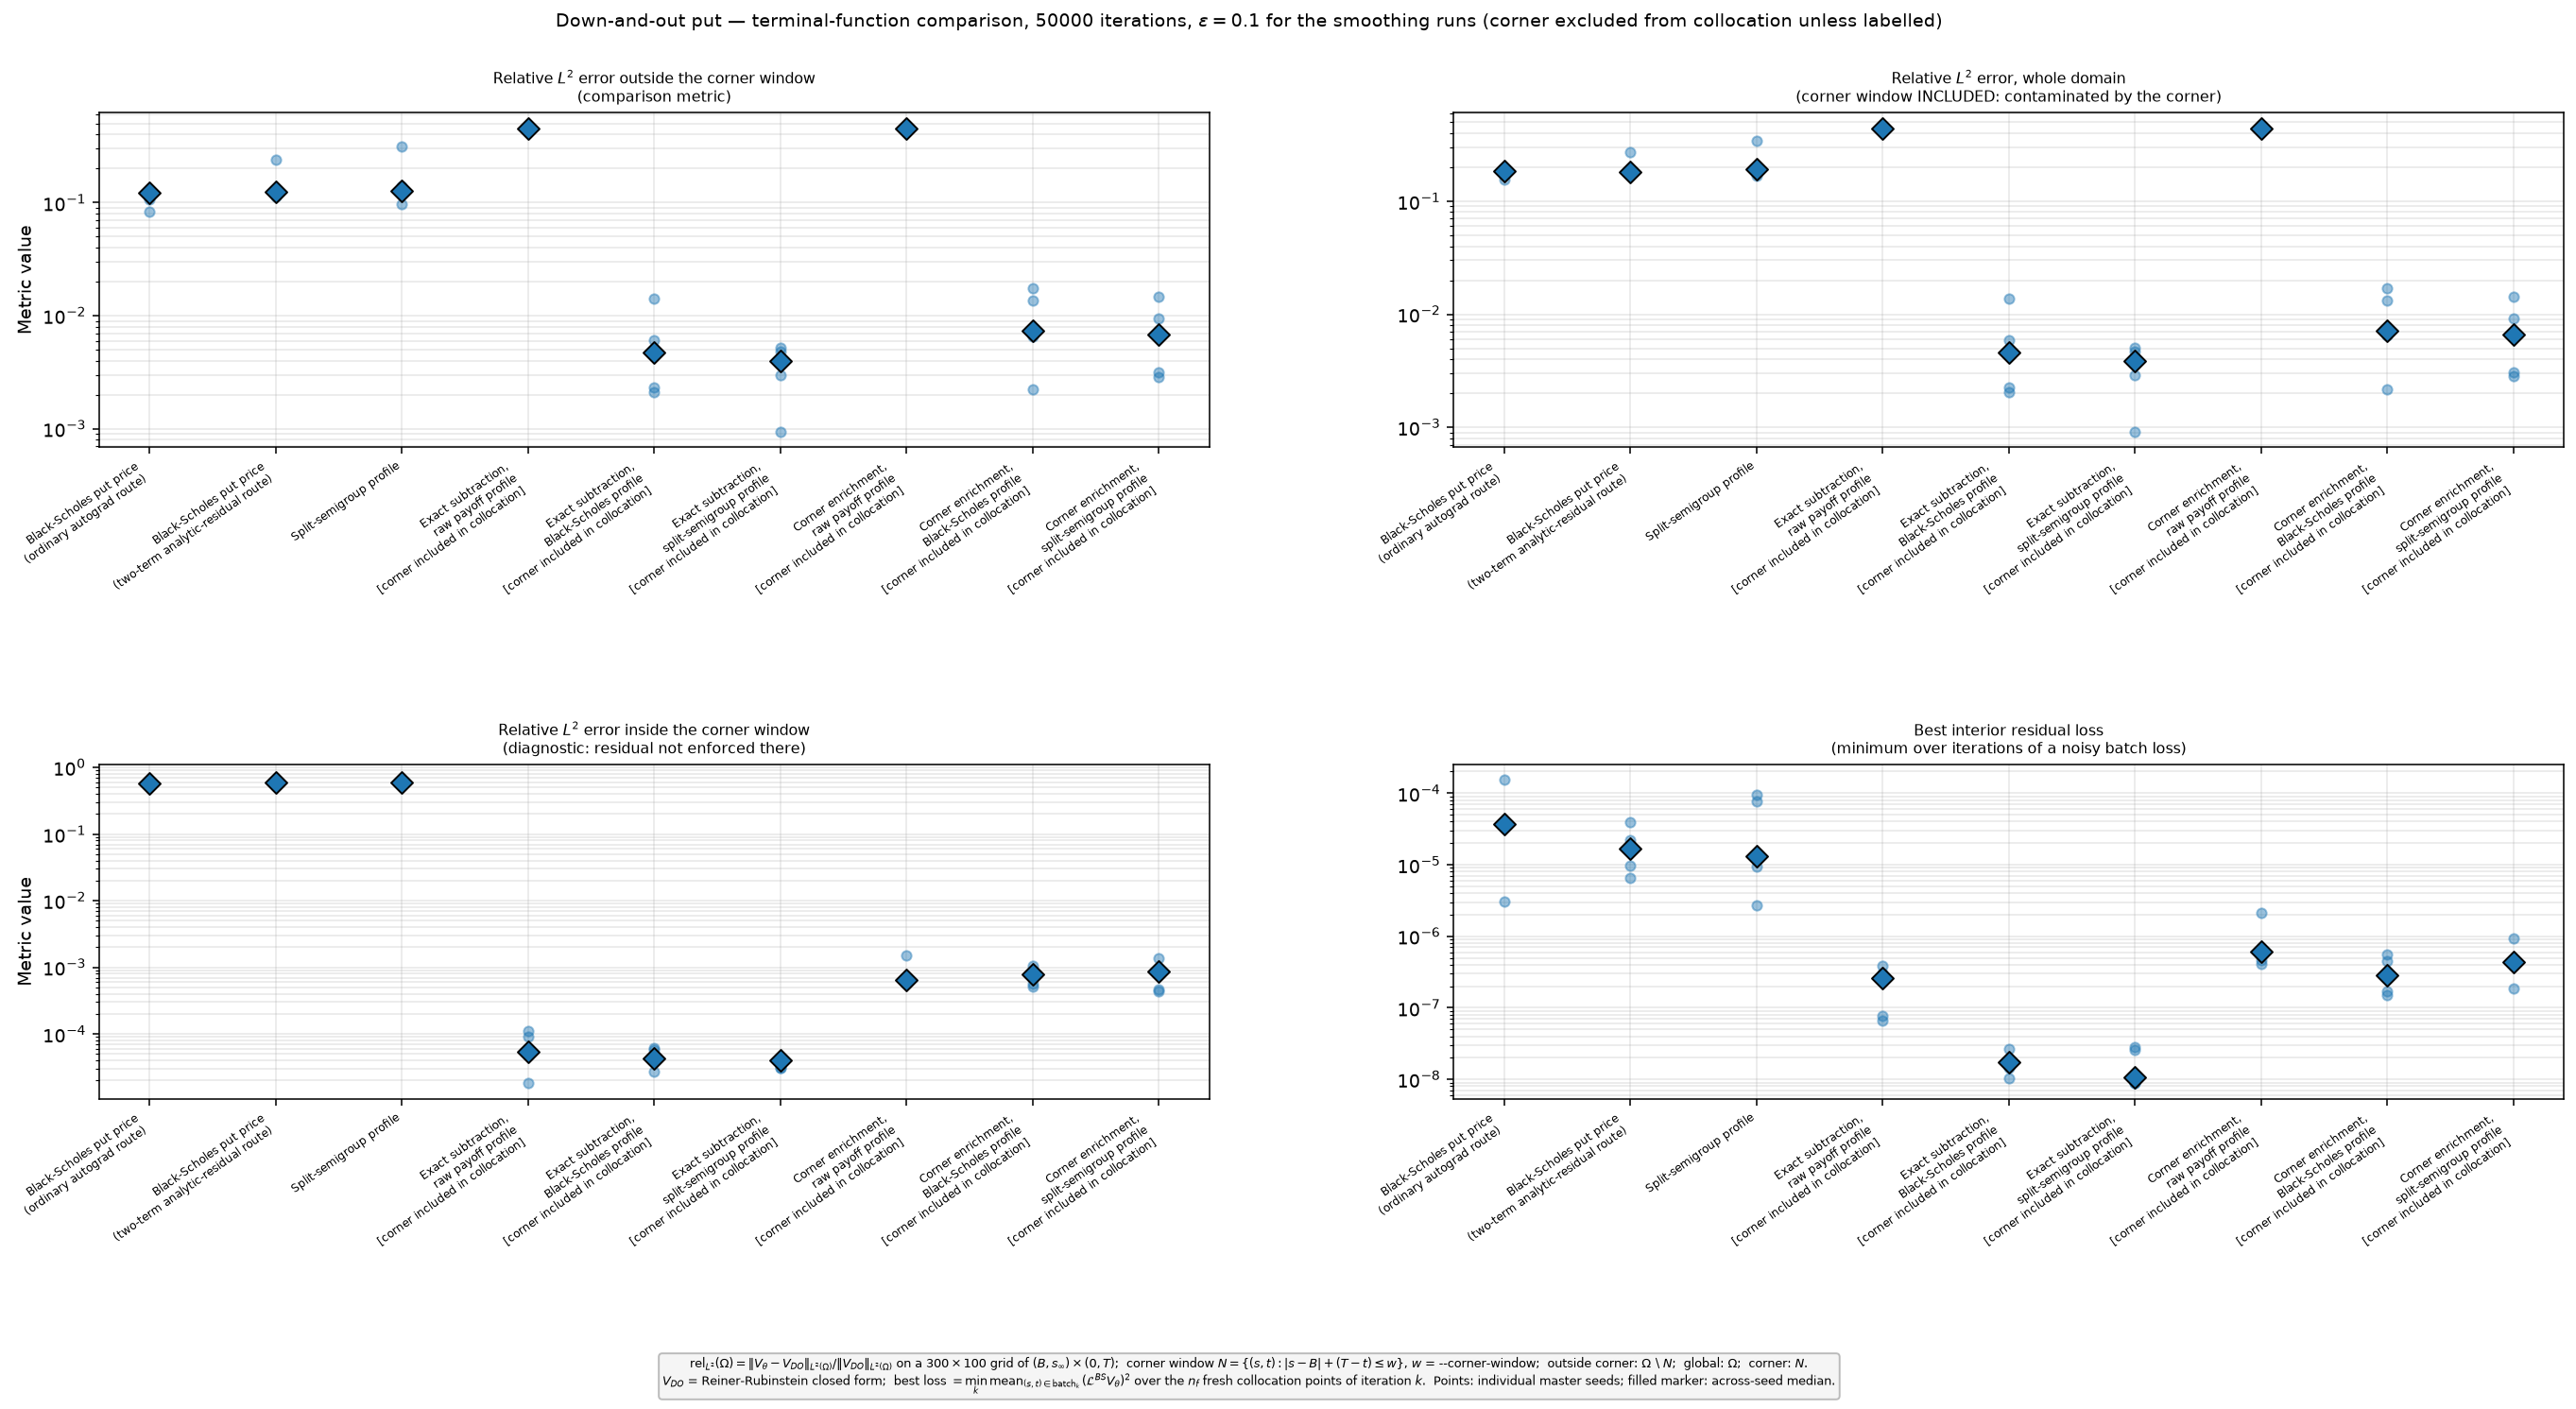
\includegraphics[width=\linewidth]{figures/terminal_function_comparison.png}
\caption{Erreur relative $L^2$ hors fenêtre de coin (métrique de comparaison), sur tout le domaine, dans la fenêtre, et meilleure perte intérieure ; 50000 itérations, $\varepsilon=0.1$ pour les runs de lissage.}
\label{fig:comparison}
\end{figure}

\begin{table}[H]
\centering
\scriptsize
\begin{adjustbox}{max width=\textwidth}
\begin{tabular}{lccccccc}
\toprule
\textbf{Configuration} & \textbf{n} & \textbf{`rel\_l2\_outside\_corner`} & \textbf{`rel\_l2\_global`} & \textbf{`rel\_l2\_corner`} & \textbf{`max\_abs\_error\_outside\_corner`} & \textbf{`best\_loss`} & \textbf{`best\_iter`} \\
\midrule
Black-Scholes put price (ordinary autograd route) & 5 & 1.218e-01 [8.310e-02, 1.305e-01] & 1.855e-01 [1.548e-01, 1.900e-01] & 5.837e-01 [5.553e-01, 6.080e-01] & 9.555e-02 [6.732e-02, 1.098e-01] & 3.675e-05 [3.035e-06, 1.548e-04] & 48150 [46551, 49611] \\
Black-Scholes put price (two-term analytic-residual route) & 5 & 1.238e-01 [1.125e-01, 2.373e-01] & 1.827e-01 [1.789e-01, 2.722e-01] & 5.958e-01 [5.678e-01, 6.094e-01] & 1.017e-01 [8.351e-02, 1.120e-01] & 1.671e-05 [6.437e-06, 3.915e-05] & 48335 [45215, 49923] \\
Split-semigroup profile & 5 & 1.270e-01 [9.763e-02, 3.113e-01] & 1.911e-01 [1.681e-01, 3.404e-01] & 5.864e-01 [5.628e-01, 6.576e-01] & 9.769e-02 [8.049e-02, 1.467e-01] & 1.299e-05 [2.730e-06, 9.448e-05] & 49474 [48150, 49879] \\
Exact subtraction, raw payoff profile & 5 & 4.549e-01 [4.537e-01, 4.559e-01] & 4.418e-01 [4.407e-01, 4.428e-01] & 5.381e-05 [1.812e-05, 1.093e-04] & 1.176e-01 [1.174e-01, 1.177e-01] & 2.581e-07 [6.530e-08, 3.878e-07] & 47907 [46834, 48332] \\
Exact subtraction, Black-Scholes profile & 5 & 4.687e-03 [2.116e-03, 1.422e-02] & 4.552e-03 [2.055e-03, 1.381e-02] & 4.335e-05 [2.693e-05, 6.171e-05] & 2.224e-03 [7.103e-04, 5.538e-03] & 1.711e-08 [1.044e-08, 2.687e-08] & 49751 [33591, 49974] \\
Exact subtraction, split-semigroup profile & 5 & 3.968e-03 [9.426e-04, 5.193e-03] & 3.854e-03 [9.156e-04, 5.044e-03] & 4.051e-05 [3.062e-05, 4.418e-05] & 1.226e-03 [2.327e-04, 1.928e-03] & 1.057e-08 [8.780e-09, 2.868e-08] & 49470 [48857, 49859] \\
Corner enrichment, raw payoff profile & 5 & 4.557e-01 [4.543e-01, 4.580e-01] & 4.426e-01 [4.412e-01, 4.449e-01] & 6.418e-04 [5.626e-04, 1.501e-03] & 1.177e-01 [1.174e-01, 1.184e-01] & 6.160e-07 [4.150e-07, 2.090e-06] & 45156 [30595, 49049] \\
Corner enrichment, Black-Scholes profile & 5 & 7.316e-03 [2.216e-03, 1.764e-02] & 7.108e-03 [2.160e-03, 1.713e-02] & 7.855e-04 [5.115e-04, 1.058e-03] & 2.979e-03 [3.960e-04, 7.044e-03] & 2.849e-07 [1.490e-07, 5.603e-07] & 49124 [20057, 49920] \\
Corner enrichment, split-semigroup profile & 5 & 6.854e-03 [2.889e-03, 1.473e-02] & 6.658e-03 [2.813e-03, 1.431e-02] & 8.729e-04 [4.331e-04, 1.359e-03] & 2.900e-03 [4.084e-04, 5.850e-03] & 4.405e-07 [1.869e-07, 9.281e-07] & 45456 [26131, 49224] \\
\bottomrule
\end{tabular}
\end{adjustbox}
\caption{Métriques par configuration, médiane [min, max] sur les graines (\texttt{table.md}).}
\label{tab:metrics}
\end{table}

\section{Diagnostics à partir des modèles sauvegardés}
\begin{figure}[H]
\centering
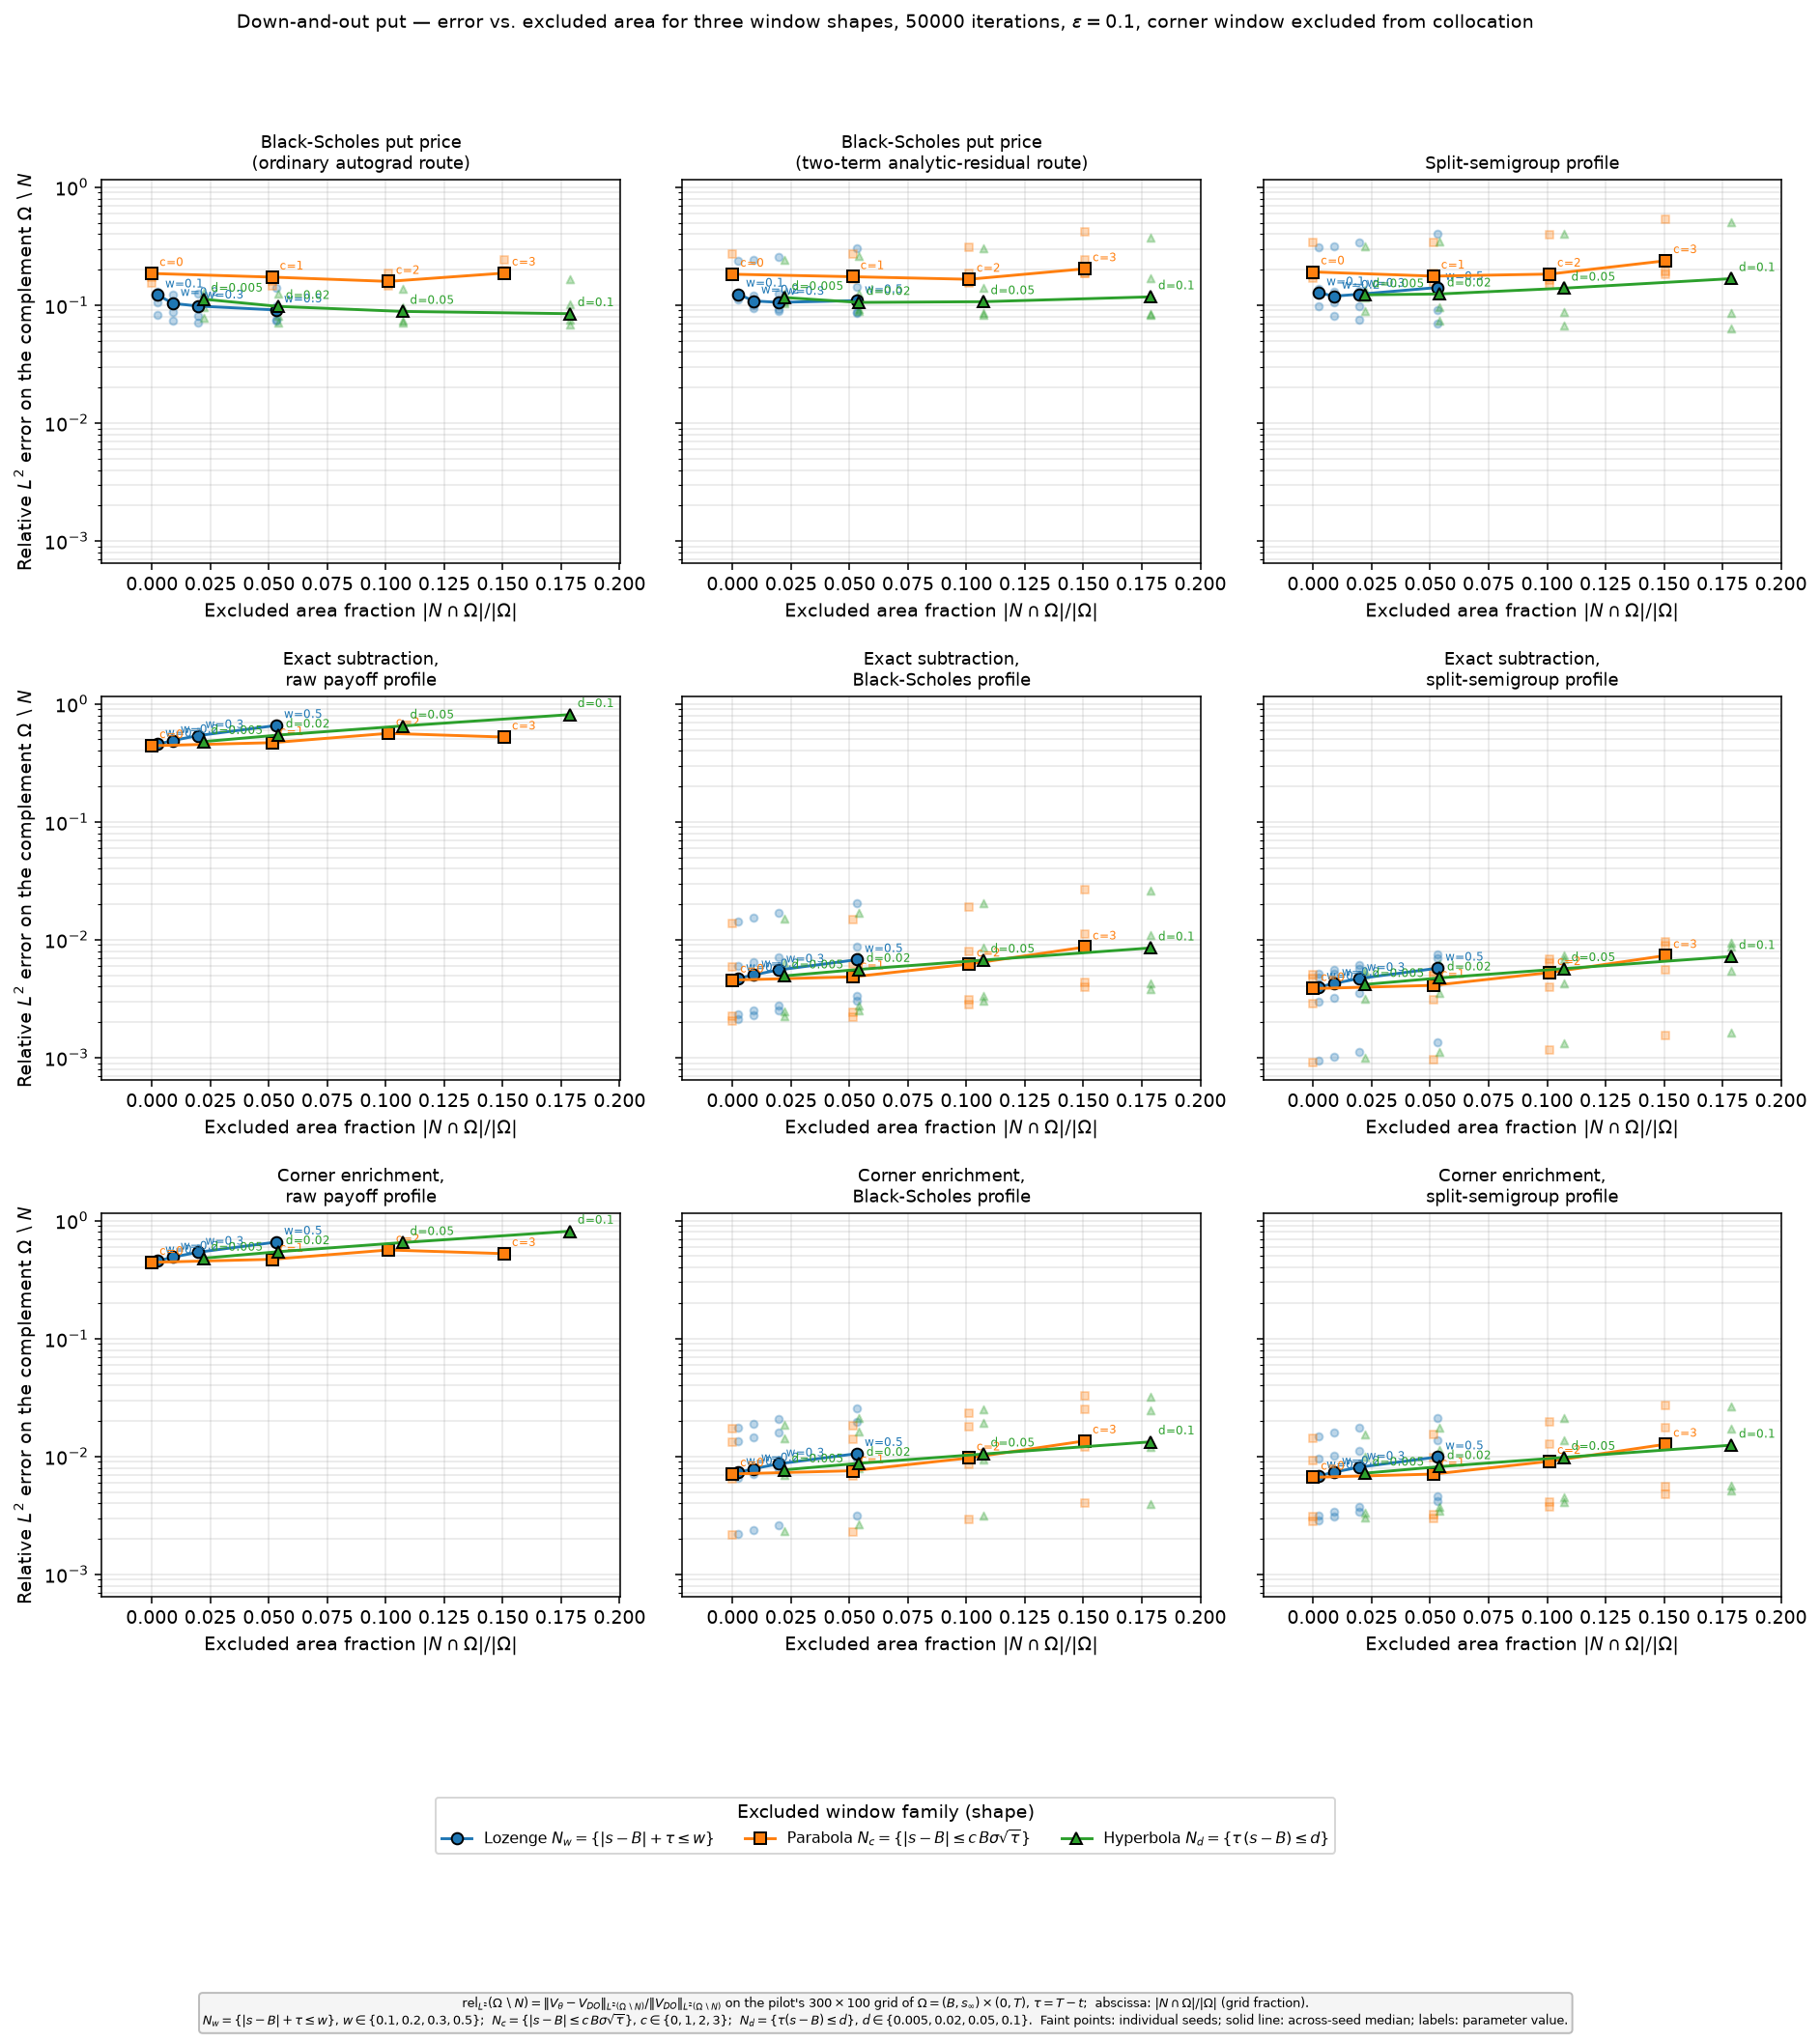
\includegraphics[width=\linewidth]{figures/rel_l2_vs_excluded_area_by_window_shape.png}
\caption{Erreur relative $L^2$ sur le complémentaire d'une fenêtre exclue autour du coin, pour trois formes de fenêtre (losange $\ell^1$, parabole, hyperbole), en fonction de la fraction d'aire exclue.}
\label{fig:window-shapes}
\end{figure}

\begin{figure}[H]
\centering
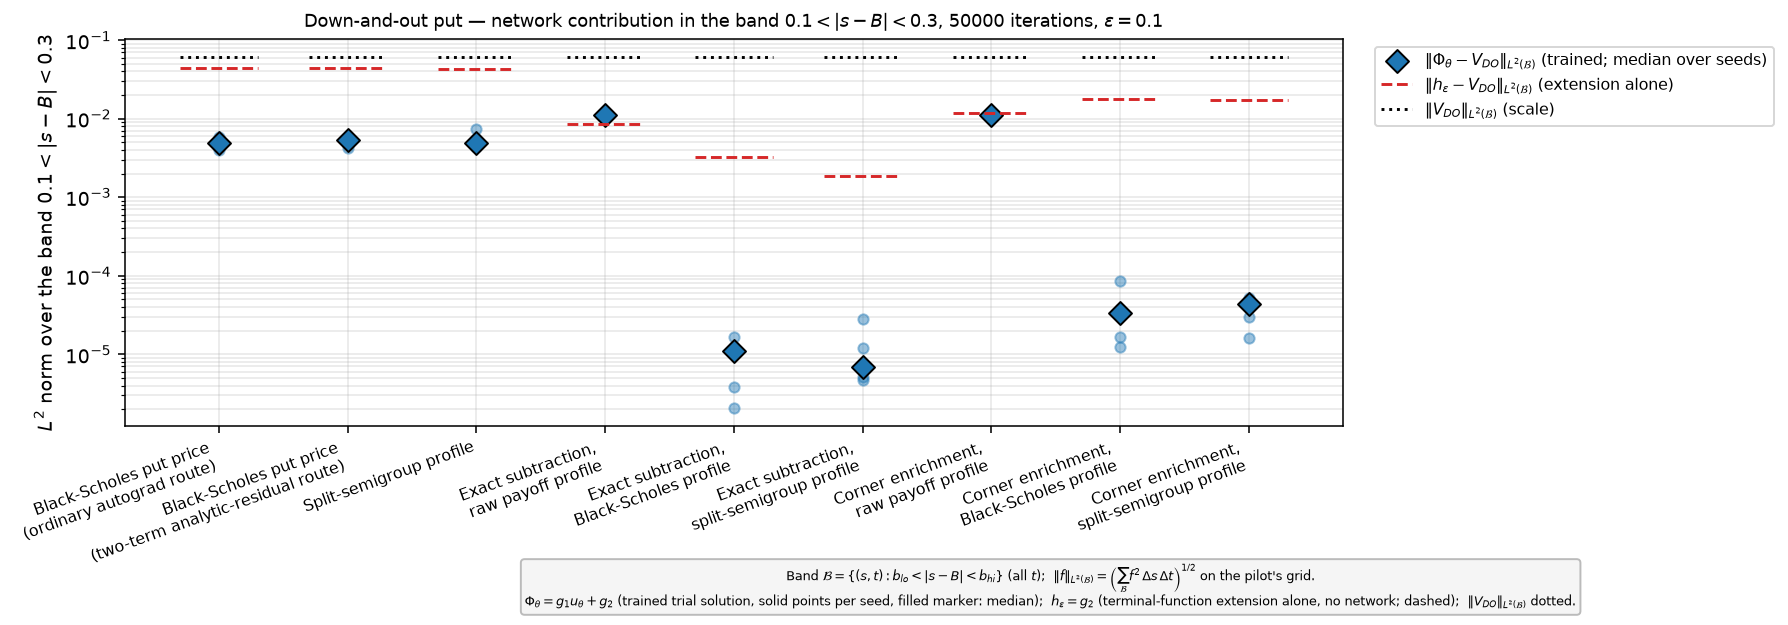
\includegraphics[width=\linewidth]{figures/band_network_contribution.png}
\caption{Bande $0.1<|s-B|<0.3$ : normes $L^2$ de $\Phi_\theta - V_{DO}$ (solution entraînée) et de $g_2 - V_{DO}$ (extension seule, sans réseau).}
\label{fig:band}
\end{figure}

\begin{table}[H]
\centering
\scriptsize
\begin{adjustbox}{max width=\textwidth}
\begin{tabular}{lcccc}
\toprule
\textbf{Configuration} & \textbf{[0.6, 0.7]} & \textbf{[0.7, 1]} & \textbf{[1, 2]} & \textbf{[2, 3]} \\
\midrule
Black-Scholes put price (ordinary autograd route) & 2.038e-01 [1.457e-01, 2.402e-01] & 7.673e-02 [6.334e-02, 9.088e-02] & 5.938e-02 [4.649e-02, 7.725e-02] & 1.335e+01 [4.184e+00, 5.720e+01] \\
Black-Scholes put price (two-term analytic-residual route) & 2.161e-01 [1.766e-01, 2.408e-01] & 8.333e-02 [6.647e-02, 9.022e-02] & 5.104e-02 [3.956e-02, 9.379e-02] & 3.335e+01 [1.031e+01, 1.359e+02] \\
Split-semigroup profile & 2.047e-01 [1.702e-01, 2.982e-01] & 7.517e-02 [6.902e-02, 1.138e-01] & 4.930e-02 [4.216e-02, 8.478e-02] & 5.675e+01 [5.935e+00, 1.823e+02] \\
Exact subtraction, raw payoff profile & 3.962e-02 [3.929e-02, 4.073e-02] & 3.397e-01 [3.389e-01, 3.409e-01] & 1.294e+00 [1.291e+00, 1.294e+00] & 6.964e+00 [2.612e+00, 9.760e+00] \\
Exact subtraction, Black-Scholes profile & 1.406e-04 [4.359e-05, 1.708e-04] & 1.831e-04 [4.396e-05, 2.910e-04] & 1.115e-03 [6.156e-04, 1.806e-03] & 3.162e+00 [1.429e+00, 9.626e+00] \\
Exact subtraction, split-semigroup profile & 1.002e-04 [8.625e-05, 3.701e-04] & 1.190e-04 [8.630e-05, 4.891e-04] & 5.204e-04 [3.707e-04, 1.733e-03] & 2.686e+00 [4.651e-01, 3.513e+00] \\
Corner enrichment, raw payoff profile & 3.947e-02 [3.912e-02, 4.072e-02] & 3.404e-01 [3.391e-01, 3.427e-01] & 1.296e+00 [1.292e+00, 1.300e+00] & 2.429e+00 [1.426e+00, 8.814e+00] \\
Corner enrichment, Black-Scholes profile & 4.394e-04 [2.012e-04, 1.088e-03] & 5.836e-04 [2.333e-04, 1.345e-03] & 1.652e-03 [1.563e-03, 2.709e-03] & 4.945e+00 [1.372e+00, 1.193e+01] \\
Corner enrichment, split-semigroup profile & 5.251e-04 [2.606e-04, 1.195e-03] & 8.443e-04 [2.944e-04, 1.164e-03] & 2.998e-03 [1.120e-03, 8.337e-03] & 4.636e+00 [1.044e+00, 9.939e+00] \\
\bottomrule
\end{tabular}
\end{adjustbox}
\caption{Erreur relative $L^2$ par bande de $s$ (tout $t$, fenêtre de coin retirée), médiane [min, max] sur les graines.}
\label{tab:bands-rel}
\end{table}

\begin{table}[H]
\centering
\scriptsize
\begin{adjustbox}{max width=\textwidth}
\begin{tabular}{lcccc}
\toprule
\textbf{Configuration} & \textbf{[0.6, 0.7]} & \textbf{[0.7, 1]} & \textbf{[1, 2]} & \textbf{[2, 3]} \\
\midrule
Black-Scholes put price (ordinary autograd route) & 6.138e-03 [4.387e-03, 7.232e-03] & 5.111e-03 [4.219e-03, 6.054e-03] & 1.193e-03 [9.339e-04, 1.552e-03] & 1.494e-03 [4.682e-04, 6.400e-03] \\
Black-Scholes put price (two-term analytic-residual route) & 6.509e-03 [5.320e-03, 7.250e-03] & 5.551e-03 [4.428e-03, 6.010e-03] & 1.025e-03 [7.948e-04, 1.884e-03] & 3.731e-03 [1.154e-03, 1.521e-02] \\
Split-semigroup profile & 6.164e-03 [5.125e-03, 8.981e-03] & 5.008e-03 [4.598e-03, 7.581e-03] & 9.903e-04 [8.471e-04, 1.703e-03] & 6.350e-03 [6.641e-04, 2.039e-02] \\
Exact subtraction, raw payoff profile & 1.193e-03 [1.183e-03, 1.227e-03] & 2.263e-02 [2.258e-02, 2.271e-02] & 2.599e-02 [2.593e-02, 2.601e-02] & 7.793e-04 [2.923e-04, 1.092e-03] \\
Exact subtraction, Black-Scholes profile & 4.234e-06 [1.313e-06, 5.143e-06] & 1.219e-05 [2.929e-06, 1.938e-05] & 2.240e-05 [1.237e-05, 3.629e-05] & 3.539e-04 [1.599e-04, 1.077e-03] \\
Exact subtraction, split-semigroup profile & 3.019e-06 [2.597e-06, 1.115e-05] & 7.929e-06 [5.749e-06, 3.258e-05] & 1.045e-05 [7.447e-06, 3.482e-05] & 3.006e-04 [5.205e-05, 3.931e-04] \\
Corner enrichment, raw payoff profile & 1.189e-03 [1.178e-03, 1.226e-03] & 2.268e-02 [2.259e-02, 2.283e-02] & 2.604e-02 [2.596e-02, 2.612e-02] & 2.718e-04 [1.596e-04, 9.863e-04] \\
Corner enrichment, Black-Scholes profile & 1.323e-05 [6.058e-06, 3.275e-05] & 3.888e-05 [1.554e-05, 8.960e-05] & 3.319e-05 [3.140e-05, 5.443e-05] & 5.533e-04 [1.535e-04, 1.335e-03] \\
Corner enrichment, split-semigroup profile & 1.581e-05 [7.846e-06, 3.597e-05] & 5.624e-05 [1.961e-05, 7.755e-05] & 6.022e-05 [2.249e-05, 1.675e-04] & 5.187e-04 [1.168e-04, 1.112e-03] \\
\bottomrule
\end{tabular}
\end{adjustbox}
\caption{Erreur absolue $L^2$ par bande de $s$ (norme discrète pondérée par l'aire des cellules).}
\label{tab:bands-abs}
\end{table}

\section{Grecques au strike}
Source : \path{data/evaluate_greeks_no_corner/20260921_corner_treatments_iters50000}. Référence : dérivée symbolique (sympy) de la forme fermée de Reiner--Rubinstein.
\begin{figure}[H]
\centering
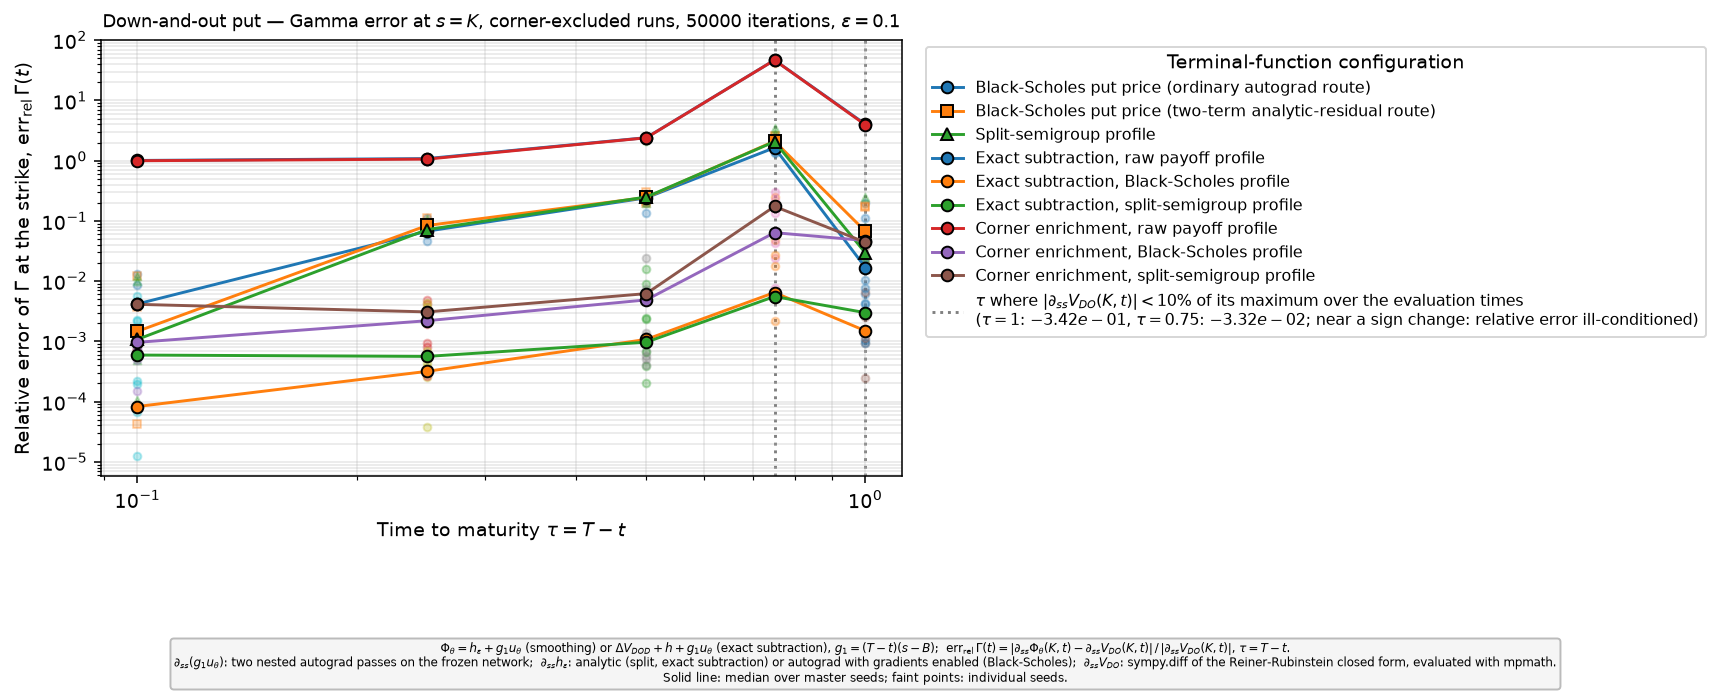
\includegraphics[width=\linewidth]{figures/greeks_no_corner.png}
\caption{Erreur relative sur $\Gamma(K,t)=\partial_{ss}\Phi_\theta(K,t)$ en fonction de $\tau=T-t$, une courbe par configuration (médiane sur les graines ; points : graines).}
\label{fig:greeks}
\end{figure}

\begin{table}[H]
\centering
\tiny
\begin{adjustbox}{max width=\textwidth}
\begin{tabular}{lccccccc}
\toprule
\textbf{Configuration} & \textbf{t} & \textbf{tau = T - t} & \textbf{Delta exact} & \textbf{Gamma exact} & \textbf{n seeds} & \textbf{err\_rel\_Delta} & \textbf{err\_rel\_Gamma} \\
\midrule
Black-Scholes put price (ordinary autograd route) & 0 & 1 & -1.4818e-01 & -3.4150e-01 (*) & 5 & 1.064e-01 [6.965e-02, 1.167e-01] & 1.679e-02 [4.303e-03, 1.986e-01] \\
Black-Scholes put price (ordinary autograd route) & 0.25 & 0.75 & -2.3063e-01 & -3.3151e-02 (*) & 5 & 1.036e-01 [8.758e-02, 1.593e-01] & 1.640e+00 [1.315e+00, 2.027e+00] \\
Black-Scholes put price (ordinary autograd route) & 0.5 & 0.5 & -3.4265e-01 & +7.9222e-01 & 5 & 8.379e-02 [7.063e-02, 1.008e-01] & 2.416e-01 [1.368e-01, 2.757e-01] \\
Black-Scholes put price (ordinary autograd route) & 0.75 & 0.25 & -4.4335e-01 & +2.4764e+00 & 5 & 2.133e-02 [1.585e-02, 4.228e-02] & 6.750e-02 [4.648e-02, 1.109e-01] \\
Black-Scholes put price (ordinary autograd route) & 0.9 & 0.1 & -4.6849e-01 & +4.1920e+00 & 5 & 2.612e-03 [9.225e-04, 1.108e-02] & 4.180e-03 [3.842e-03, 1.333e-02] \\
Black-Scholes put price (two-term analytic-residual route) & 0 & 1 & -1.4818e-01 & -3.4150e-01 (*) & 5 & 1.355e-01 [7.518e-02, 1.415e-01] & 6.690e-02 [2.020e-02, 1.776e-01] \\
Black-Scholes put price (two-term analytic-residual route) & 0.25 & 0.75 & -2.3063e-01 & -3.3151e-02 (*) & 5 & 1.071e-01 [8.129e-02, 1.165e-01] & 2.104e+00 [1.778e+00, 2.610e+00] \\
Black-Scholes put price (two-term analytic-residual route) & 0.5 & 0.5 & -3.4265e-01 & +7.9222e-01 & 5 & 8.199e-02 [6.495e-02, 8.626e-02] & 2.449e-01 [2.016e-01, 3.001e-01] \\
Black-Scholes put price (two-term analytic-residual route) & 0.75 & 0.25 & -4.4335e-01 & +2.4764e+00 & 5 & 2.621e-02 [2.055e-02, 3.734e-02] & 8.384e-02 [6.869e-02, 1.122e-01] \\
Black-Scholes put price (two-term analytic-residual route) & 0.9 & 0.1 & -4.6849e-01 & +4.1920e+00 & 5 & 1.601e-03 [4.936e-05, 6.331e-03] & 1.467e-03 [4.283e-05, 1.203e-02] \\
Split-semigroup profile & 0 & 1 & -1.4818e-01 & -3.4150e-01 (*) & 5 & 1.003e-01 [1.493e-02, 1.438e-01] & 2.924e-02 [2.166e-02, 2.517e-01] \\
Split-semigroup profile & 0.25 & 0.75 & -2.3063e-01 & -3.3151e-02 (*) & 5 & 9.237e-02 [4.905e-02, 1.468e-01] & 2.068e+00 [1.823e+00, 3.518e+00] \\
Split-semigroup profile & 0.5 & 0.5 & -3.4265e-01 & +7.9222e-01 & 5 & 7.916e-02 [5.065e-02, 1.251e-01] & 2.490e-01 [1.980e-01, 2.781e-01] \\
Split-semigroup profile & 0.75 & 0.25 & -4.4335e-01 & +2.4764e+00 & 5 & 2.505e-02 [1.876e-02, 2.705e-02] & 7.167e-02 [6.584e-02, 1.075e-01] \\
Split-semigroup profile & 0.9 & 0.1 & -4.6849e-01 & +4.1920e+00 & 5 & 4.039e-04 [2.811e-04, 2.158e-03] & 1.078e-03 [1.043e-04, 1.212e-02] \\
Exact subtraction, raw payoff profile & 0 & 1 & -1.4818e-01 & -3.4150e-01 (*) & 5 & 3.228e+00 [3.225e+00, 3.240e+00] & 4.017e+00 [3.574e+00, 4.073e+00] \\
Exact subtraction, raw payoff profile & 0.25 & 0.75 & -2.3063e-01 & -3.3151e-02 (*) & 5 & 2.088e+00 [2.085e+00, 2.095e+00] & 4.681e+01 [4.250e+01, 4.806e+01] \\
Exact subtraction, raw payoff profile & 0.5 & 0.5 & -3.4265e-01 & +7.9222e-01 & 5 & 1.416e+00 [1.413e+00, 1.418e+00] & 2.411e+00 [2.150e+00, 2.451e+00] \\
Exact subtraction, raw payoff profile & 0.75 & 0.25 & -4.4335e-01 & +2.4764e+00 & 5 & 1.103e+00 [1.101e+00, 1.105e+00] & 1.083e+00 [9.903e-01, 1.099e+00] \\
Exact subtraction, raw payoff profile & 0.9 & 0.1 & -4.6849e-01 & +4.1920e+00 & 5 & 1.052e+00 [1.050e+00, 1.053e+00] & 1.008e+00 [9.435e-01, 1.019e+00] \\
Exact subtraction, Black-Scholes profile & 0 & 1 & -1.4818e-01 & -3.4150e-01 (*) & 5 & 1.549e-04 [8.349e-05, 6.463e-04] & 1.490e-03 [2.459e-04, 6.698e-03] \\
Exact subtraction, Black-Scholes profile & 0.25 & 0.75 & -2.3063e-01 & -3.3151e-02 (*) & 5 & 1.472e-04 [1.853e-06, 6.461e-04] & 6.462e-03 [6.078e-03, 2.409e-02] \\
Exact subtraction, Black-Scholes profile & 0.5 & 0.5 & -3.4265e-01 & +7.9222e-01 & 5 & 2.426e-04 [5.164e-06, 3.615e-04] & 1.076e-03 [5.006e-04, 1.351e-03] \\
Exact subtraction, Black-Scholes profile & 0.75 & 0.25 & -4.4335e-01 & +2.4764e+00 & 5 & 7.842e-05 [2.869e-05, 3.811e-04] & 3.171e-04 [3.742e-05, 4.418e-04] \\
Exact subtraction, Black-Scholes profile & 0.9 & 0.1 & -4.6849e-01 & +4.1920e+00 & 5 & 7.921e-05 [2.017e-05, 1.380e-04] & 8.269e-05 [1.223e-05, 2.208e-04] \\
Exact subtraction, split-semigroup profile & 0 & 1 & -1.4818e-01 & -3.4150e-01 (*) & 5 & 3.002e-04 [1.269e-04, 7.926e-04] & 2.990e-03 [9.200e-04, 1.035e-02] \\
Exact subtraction, split-semigroup profile & 0.25 & 0.75 & -2.3063e-01 & -3.3151e-02 (*) & 5 & 1.656e-04 [3.019e-05, 4.315e-04] & 5.542e-03 [2.196e-03, 5.806e-02] \\
Exact subtraction, split-semigroup profile & 0.5 & 0.5 & -3.4265e-01 & +7.9222e-01 & 5 & 2.074e-04 [1.060e-04, 5.968e-04] & 9.687e-04 [3.884e-04, 2.451e-03] \\
Exact subtraction, split-semigroup profile & 0.75 & 0.25 & -4.4335e-01 & +2.4764e+00 & 5 & 1.640e-04 [4.401e-05, 3.802e-04] & 5.615e-04 [3.282e-04, 9.357e-04] \\
Exact subtraction, split-semigroup profile & 0.9 & 0.1 & -4.6849e-01 & +4.1920e+00 & 5 & 1.923e-04 [9.877e-05, 5.444e-04] & 5.914e-04 [1.495e-04, 1.274e-03] \\
Corner enrichment, raw payoff profile & 0 & 1 & -1.4818e-01 & -3.4150e-01 (*) & 5 & 3.232e+00 [3.215e+00, 3.246e+00] & 3.929e+00 [3.583e+00, 4.319e+00] \\
Corner enrichment, raw payoff profile & 0.25 & 0.75 & -2.3063e-01 & -3.3151e-02 (*) & 5 & 2.092e+00 [2.080e+00, 2.101e+00] & 4.672e+01 [4.584e+01, 4.743e+01] \\
Corner enrichment, raw payoff profile & 0.5 & 0.5 & -3.4265e-01 & +7.9222e-01 & 5 & 1.418e+00 [1.411e+00, 1.420e+00] & 2.396e+00 [2.259e+00, 2.438e+00] \\
Corner enrichment, raw payoff profile & 0.75 & 0.25 & -4.4335e-01 & +2.4764e+00 & 5 & 1.105e+00 [1.104e+00, 1.106e+00] & 1.060e+00 [1.032e+00, 1.081e+00] \\
Corner enrichment, raw payoff profile & 0.9 & 0.1 & -4.6849e-01 & +4.1920e+00 & 5 & 1.052e+00 [1.041e+00, 1.054e+00] & 9.978e-01 [9.804e-01, 1.018e+00] \\
Corner enrichment, Black-Scholes profile & 0 & 1 & -1.4818e-01 & -3.4150e-01 (*) & 5 & 1.388e-03 [6.775e-04, 1.661e-03] & 4.714e-02 [7.676e-03, 1.132e-01] \\
Corner enrichment, Black-Scholes profile & 0.25 & 0.75 & -2.3063e-01 & -3.3151e-02 (*) & 5 & 7.944e-04 [1.927e-05, 1.635e-03] & 6.375e-02 [1.802e-02, 2.470e-01] \\
Corner enrichment, Black-Scholes profile & 0.5 & 0.5 & -3.4265e-01 & +7.9222e-01 & 5 & 1.193e-03 [5.798e-05, 1.880e-03] & 4.873e-03 [2.039e-04, 1.618e-02] \\
Corner enrichment, Black-Scholes profile & 0.75 & 0.25 & -4.4335e-01 & +2.4764e+00 & 5 & 7.177e-04 [2.937e-04, 1.987e-03] & 2.198e-03 [2.634e-04, 4.902e-03] \\
Corner enrichment, Black-Scholes profile & 0.9 & 0.1 & -4.6849e-01 & +4.1920e+00 & 5 & 6.028e-04 [3.209e-05, 7.496e-04] & 9.626e-04 [7.398e-04, 1.694e-03] \\
Corner enrichment, split-semigroup profile & 0 & 1 & -1.4818e-01 & -3.4150e-01 (*) & 5 & 3.539e-03 [1.628e-03, 6.720e-03] & 4.405e-02 [1.123e-03, 7.510e-02] \\
Corner enrichment, split-semigroup profile & 0.25 & 0.75 & -2.3063e-01 & -3.3151e-02 (*) & 5 & 8.760e-04 [9.496e-05, 3.735e-03] & 1.740e-01 [4.253e-02, 3.060e-01] \\
Corner enrichment, split-semigroup profile & 0.5 & 0.5 & -3.4265e-01 & +7.9222e-01 & 5 & 8.006e-04 [2.709e-04, 2.185e-03] & 6.199e-03 [4.043e-04, 2.404e-02] \\
Corner enrichment, split-semigroup profile & 0.75 & 0.25 & -4.4335e-01 & +2.4764e+00 & 5 & 6.953e-04 [2.344e-04, 2.595e-03] & 3.079e-03 [6.961e-04, 4.406e-03] \\
Corner enrichment, split-semigroup profile & 0.9 & 0.1 & -4.6849e-01 & +4.1920e+00 & 5 & 1.589e-03 [1.576e-04, 1.871e-03] & 4.114e-03 [2.167e-03, 5.759e-03] \\
\bottomrule
\end{tabular}
\end{adjustbox}
\caption{$\Delta$ et $\Gamma$ au strike : erreur relative ponctuelle, médiane [min, max] sur les graines ; (*) marque un $\Gamma$ exact proche d'un changement de signe.}
\label{tab:greeks}
\end{table}

\section{Figures par run (graine 0)}
\subsection{Black-Scholes put price (ordinary autograd route)}
lissage du coin, profil Black--Scholes $V^e$, route autograd ordinaire. Run : \path{20260913_045605_iters50000_eps0.1_seed0_blackscholes_nocorner}.
\begin{figure}[H]
\centering
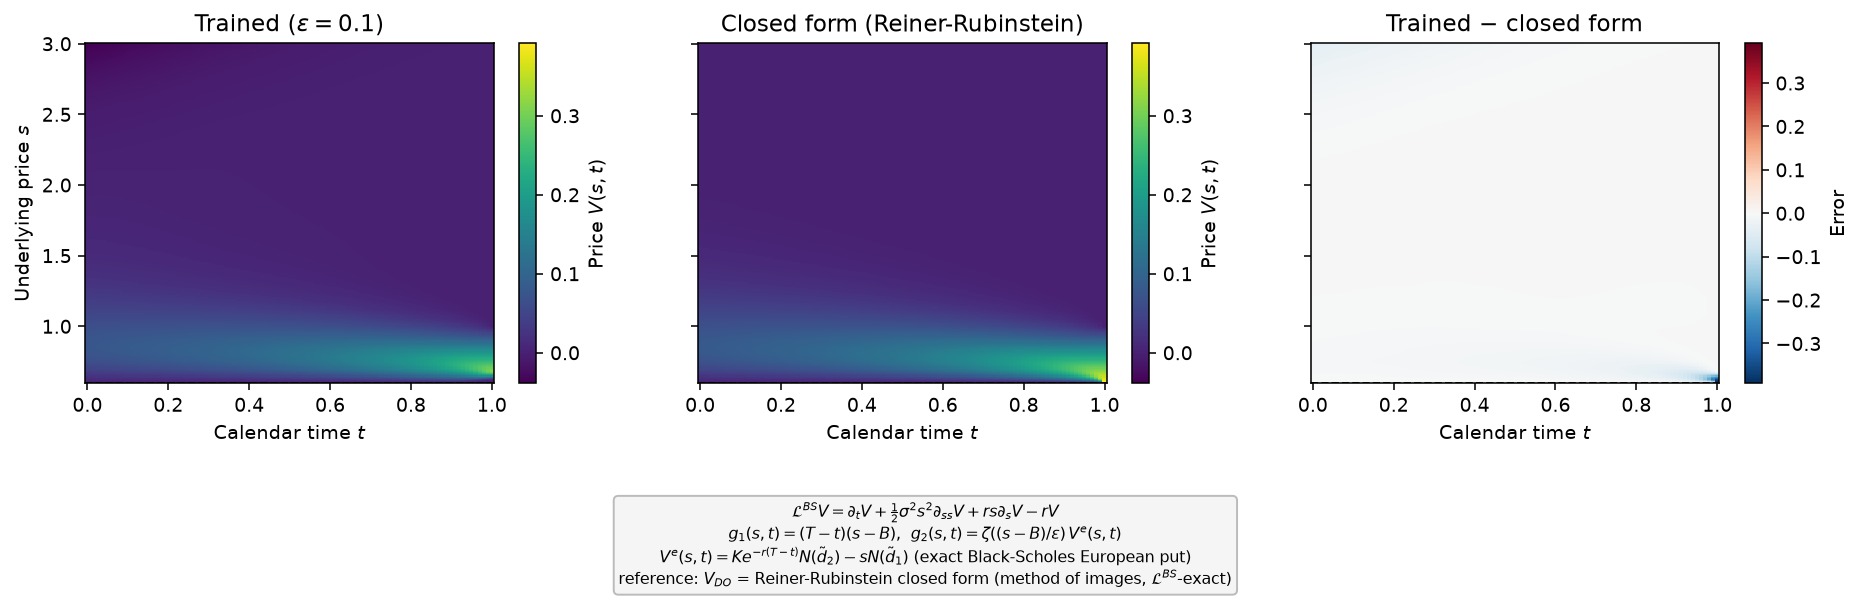
\includegraphics[width=\linewidth]{figures/blackscholes_seed0_price_surface_eps0.1.png}
\caption{Surface de prix : solution entraînée, forme fermée, différence. lissage du coin, profil Black--Scholes $V^e$, route autograd ordinaire.}
\label{fig:blackscholes-price_surface_eps0.1}
\end{figure}

\begin{figure}[H]
\centering
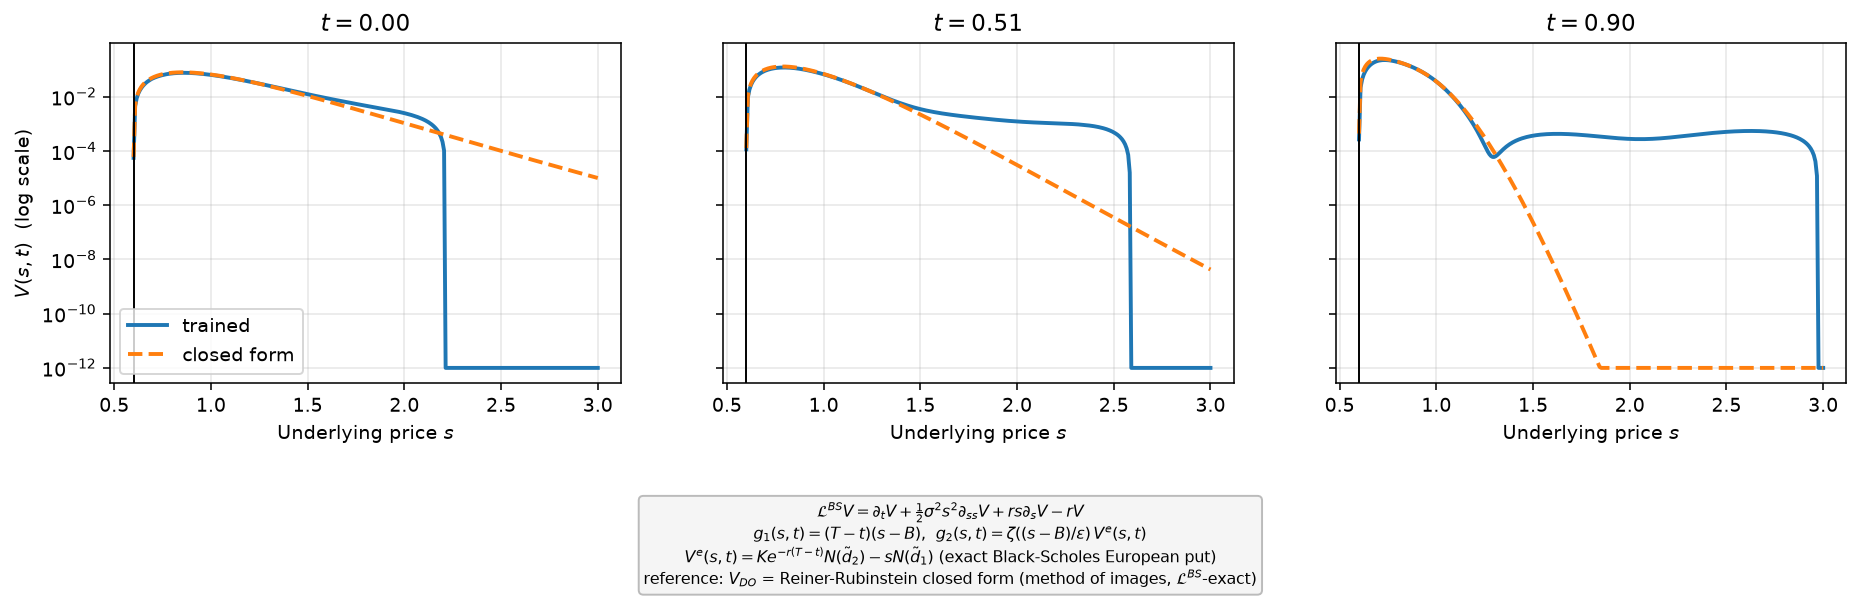
\includegraphics[width=\linewidth]{figures/blackscholes_seed0_log_slice_eps0.1.png}
\caption{Coupes $V(s,t)$ à $t$ fixé, échelle logarithmique (solution entraînée en trait plein, forme fermée en tirets). lissage du coin, profil Black--Scholes $V^e$, route autograd ordinaire.}
\label{fig:blackscholes-log_slice_eps0.1}
\end{figure}

\subsection{Black-Scholes put price (two-term analytic-residual route)}
lissage du coin, profil Black--Scholes $V^e$, route analytique à deux termes. Run : \path{20260913_035016_iters50000_eps0.1_seed0_blackscholes_analyticres_nocorner}.
\begin{figure}[H]
\centering
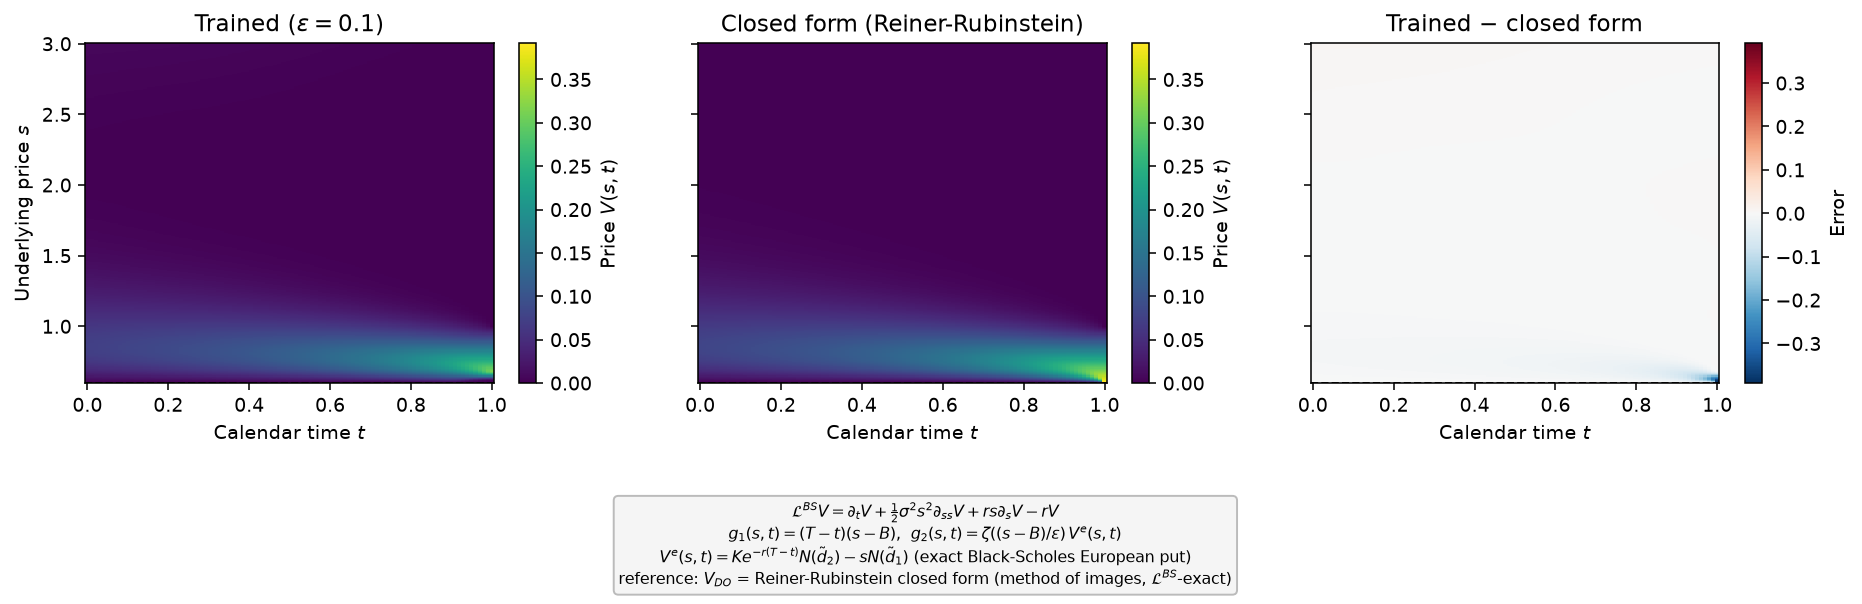
\includegraphics[width=\linewidth]{figures/blackscholes_analyticres_seed0_price_surface_eps0.1.png}
\caption{Surface de prix : solution entraînée, forme fermée, différence. lissage du coin, profil Black--Scholes $V^e$, route analytique à deux termes.}
\label{fig:blackscholes_analyticres-price_surface_eps0.1}
\end{figure}

\begin{figure}[H]
\centering
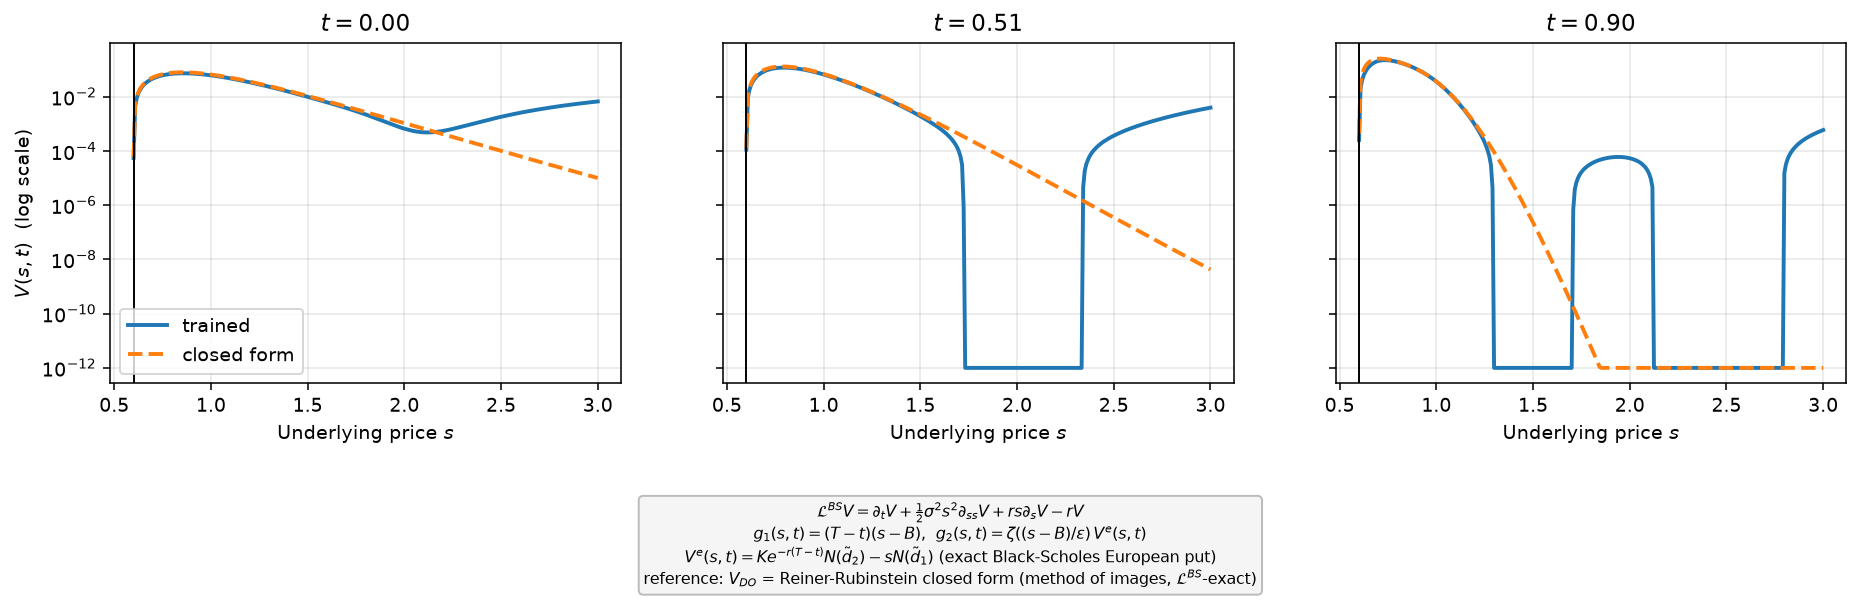
\includegraphics[width=\linewidth]{figures/blackscholes_analyticres_seed0_log_slice_eps0.1.png}
\caption{Coupes $V(s,t)$ à $t$ fixé, échelle logarithmique (solution entraînée en trait plein, forme fermée en tirets). lissage du coin, profil Black--Scholes $V^e$, route analytique à deux termes.}
\label{fig:blackscholes_analyticres-log_slice_eps0.1}
\end{figure}

\subsection{Split-semigroup profile}
lissage du coin, profil split-semigroupe. Run : \path{20260912_071515_iters50000_eps0.1_seed0_split_nuc0.3_nquad8000_nocorner}.
\begin{figure}[H]
\centering
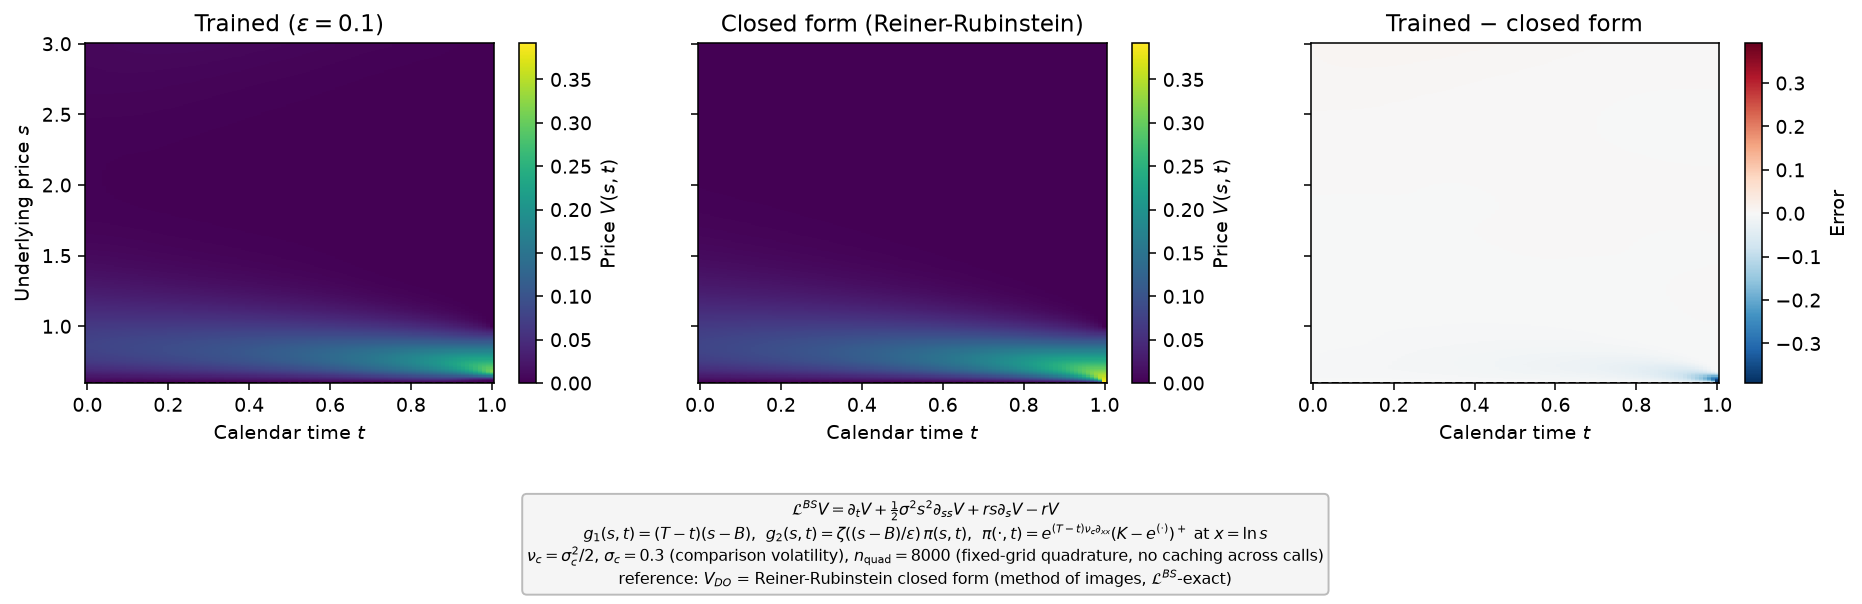
\includegraphics[width=\linewidth]{figures/split_seed0_price_surface_eps0.1.png}
\caption{Surface de prix : solution entraînée, forme fermée, différence. lissage du coin, profil split-semigroupe.}
\label{fig:split-price_surface_eps0.1}
\end{figure}

\begin{figure}[H]
\centering
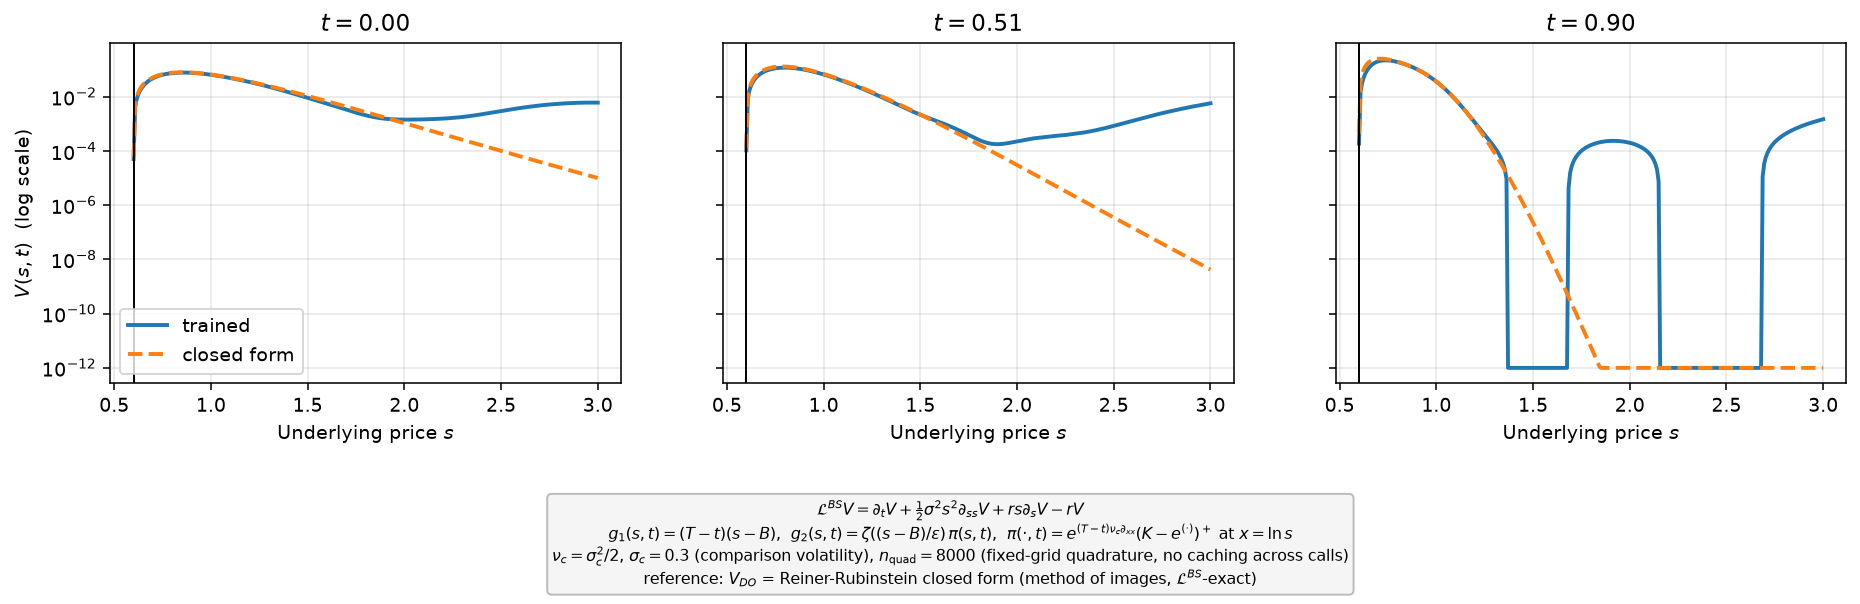
\includegraphics[width=\linewidth]{figures/split_seed0_log_slice_eps0.1.png}
\caption{Coupes $V(s,t)$ à $t$ fixé, échelle logarithmique (solution entraînée en trait plein, forme fermée en tirets). lissage du coin, profil split-semigroupe.}
\label{fig:split-log_slice_eps0.1}
\end{figure}

\subsection{Exact subtraction, raw payoff profile}
soustraction exacte ($\Delta V_{DOD}$), profil payoff brut (contrôle négatif). Run : \path{20260920_201745_iters50000_eps0_seed0_subtraction_raw}.
\begin{figure}[H]
\centering
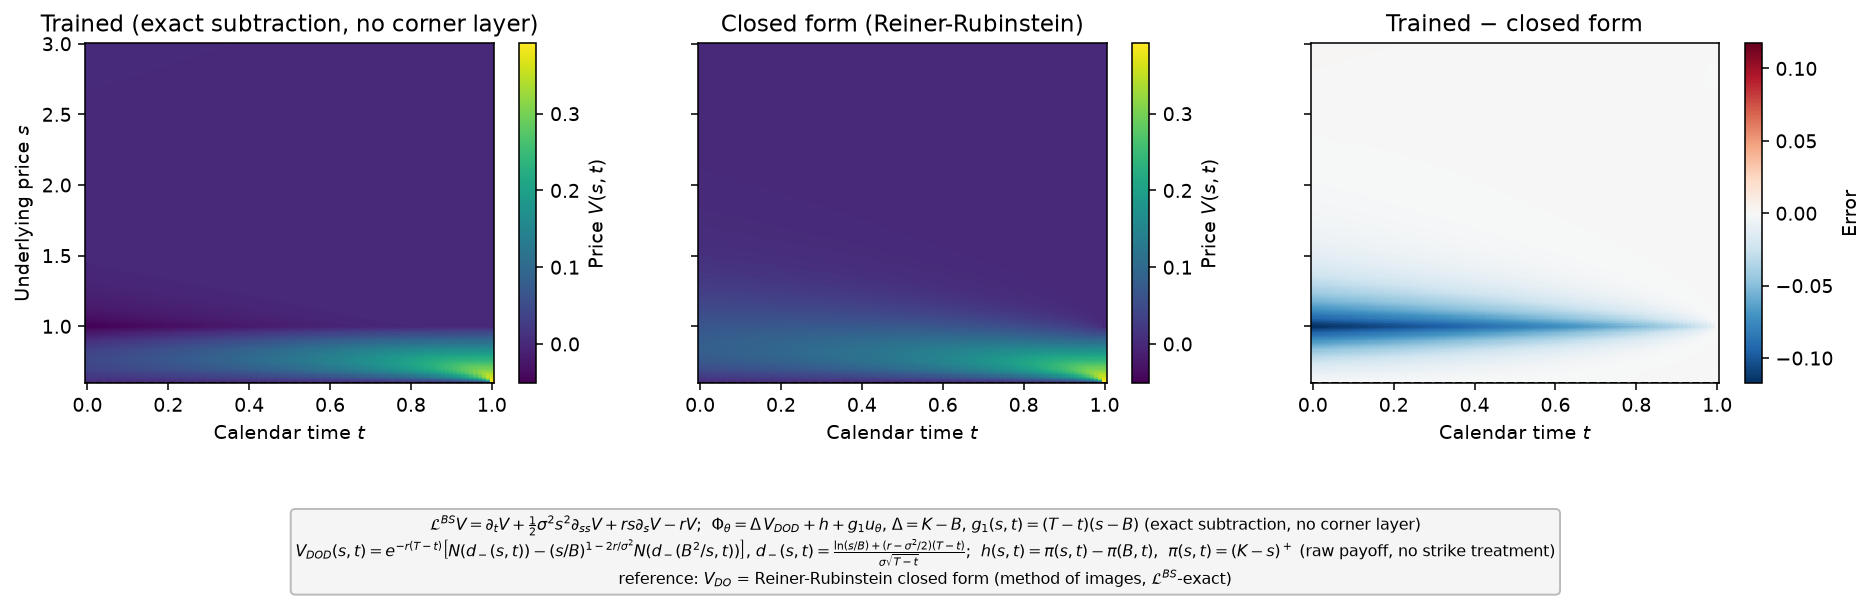
\includegraphics[width=\linewidth]{figures/subtraction_raw_seed0_price_surface_eps0.png}
\caption{Surface de prix : solution entraînée, forme fermée, différence. soustraction exacte ($\Delta V_{DOD}$), profil payoff brut (contrôle négatif).}
\label{fig:subtraction_raw-price_surface_eps0}
\end{figure}

\begin{figure}[H]
\centering
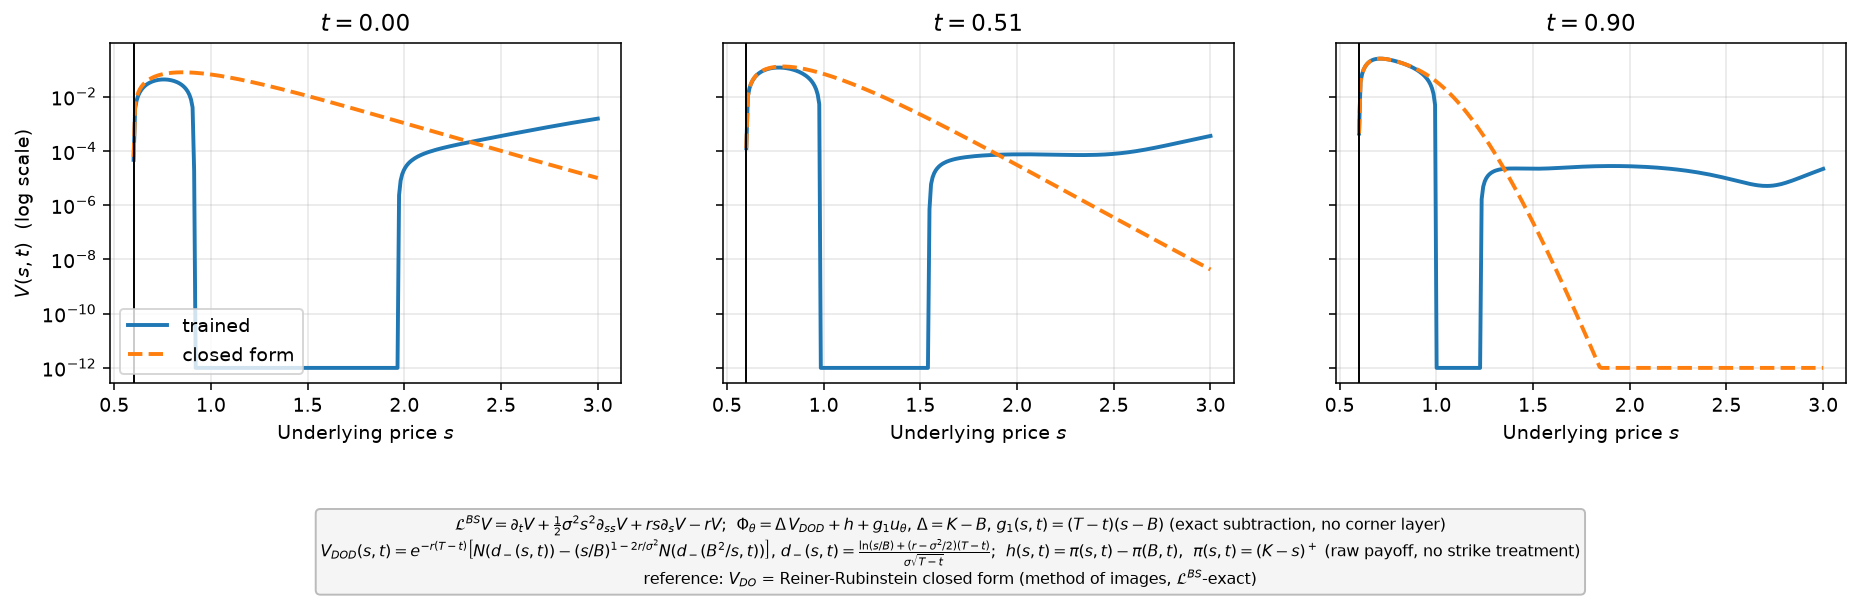
\includegraphics[width=\linewidth]{figures/subtraction_raw_seed0_log_slice_eps0.png}
\caption{Coupes $V(s,t)$ à $t$ fixé, échelle logarithmique (solution entraînée en trait plein, forme fermée en tirets). soustraction exacte ($\Delta V_{DOD}$), profil payoff brut (contrôle négatif).}
\label{fig:subtraction_raw-log_slice_eps0}
\end{figure}

\begin{figure}[H]
\centering
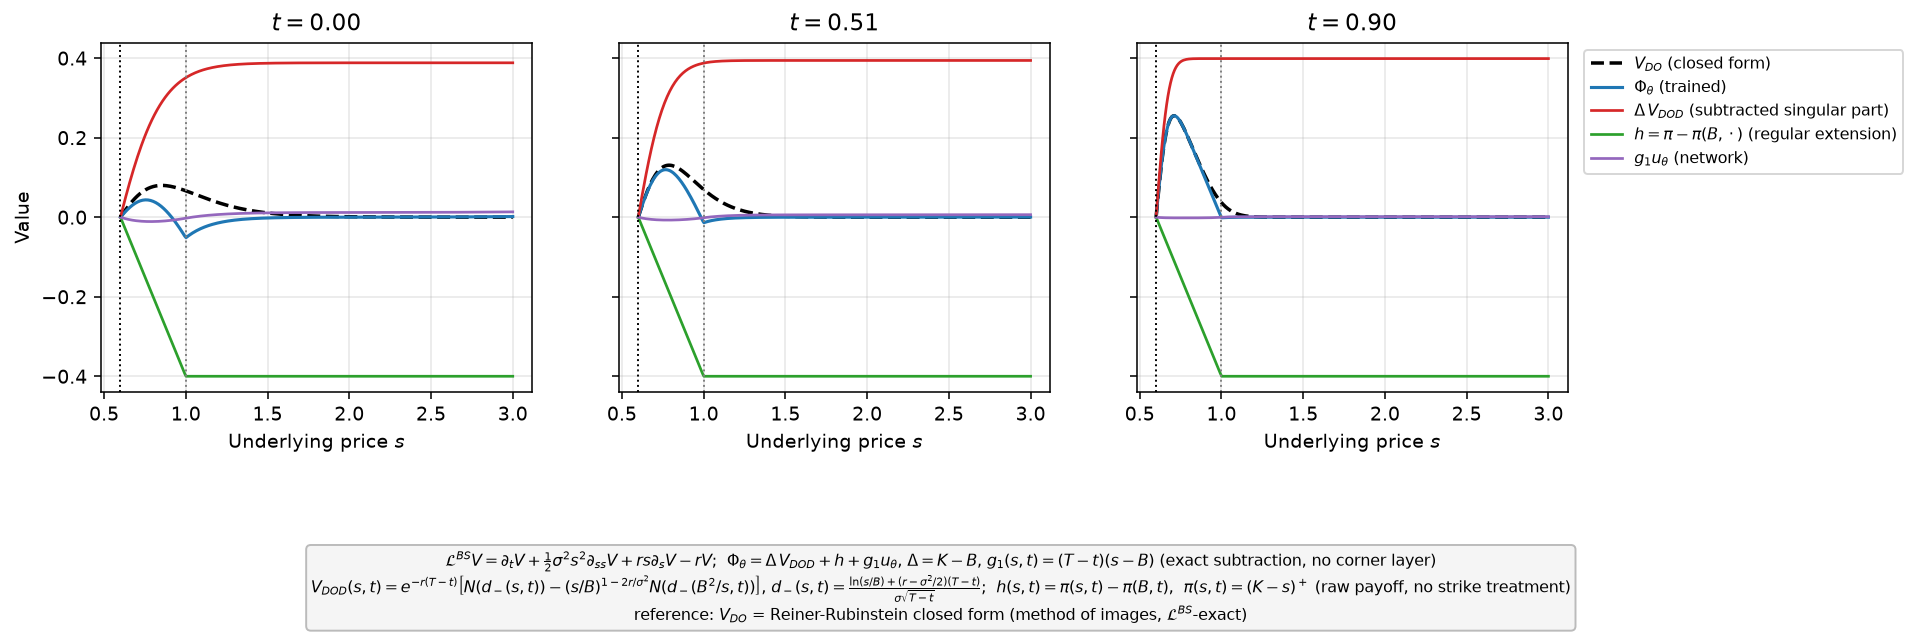
\includegraphics[width=\linewidth]{figures/subtraction_raw_seed0_subtraction_decomposition.png}
\caption{Décomposition de l'estimateur : partie singulière en forme fermée, extension régulière $h$, réseau $g_1u_\theta$, total, contre $V_{DO}$. soustraction exacte ($\Delta V_{DOD}$), profil payoff brut (contrôle négatif).}
\label{fig:subtraction_raw-subtraction_decomposition}
\end{figure}

\subsection{Exact subtraction, Black-Scholes profile}
soustraction exacte ($\Delta V_{DOD}$), profil Black--Scholes $V^e$. Run : \path{20260920_201746_iters50000_eps0_seed0_subtraction_blackscholes}.
\begin{figure}[H]
\centering
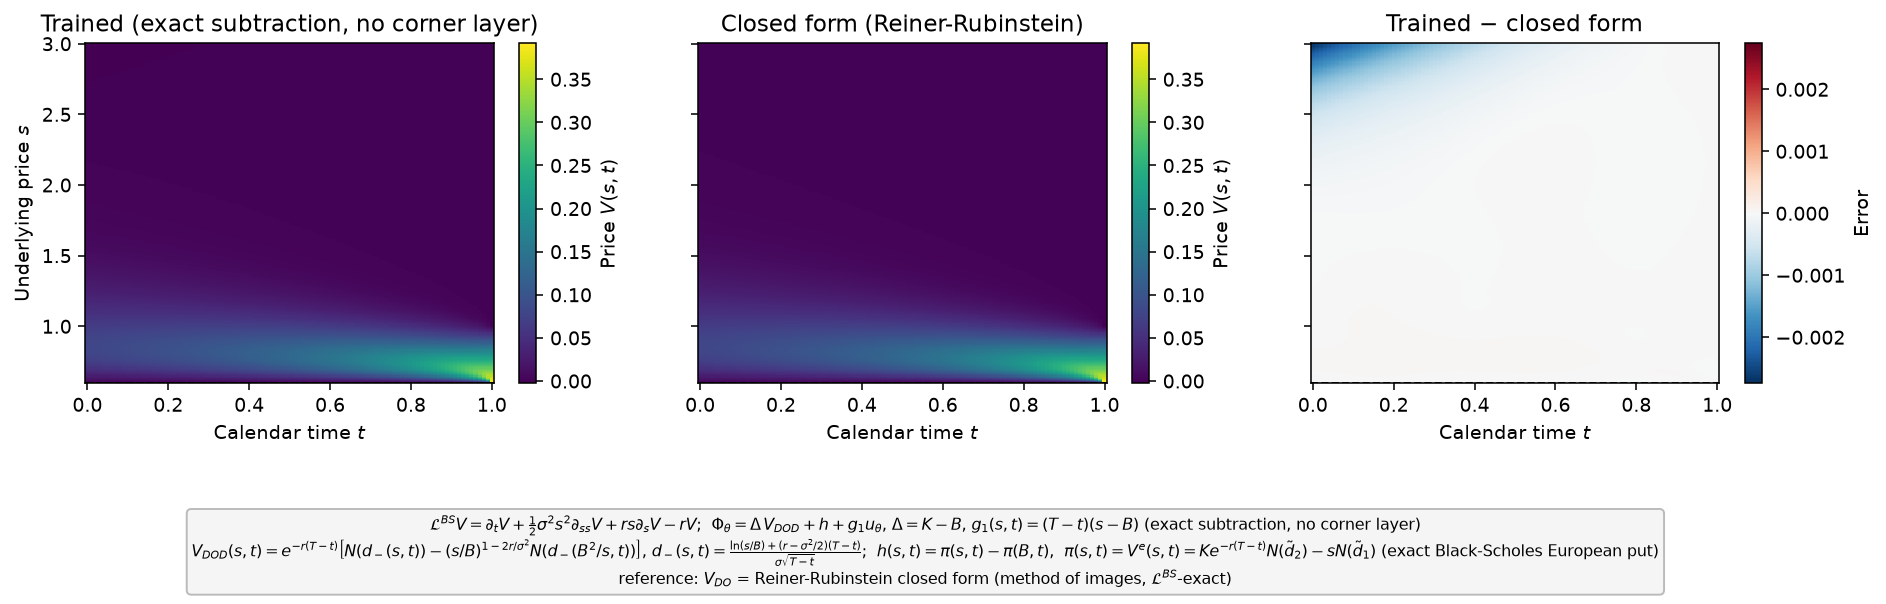
\includegraphics[width=\linewidth]{figures/subtraction_blackscholes_seed0_price_surface_eps0.png}
\caption{Surface de prix : solution entraînée, forme fermée, différence. soustraction exacte ($\Delta V_{DOD}$), profil Black--Scholes $V^e$.}
\label{fig:subtraction_blackscholes-price_surface_eps0}
\end{figure}

\begin{figure}[H]
\centering
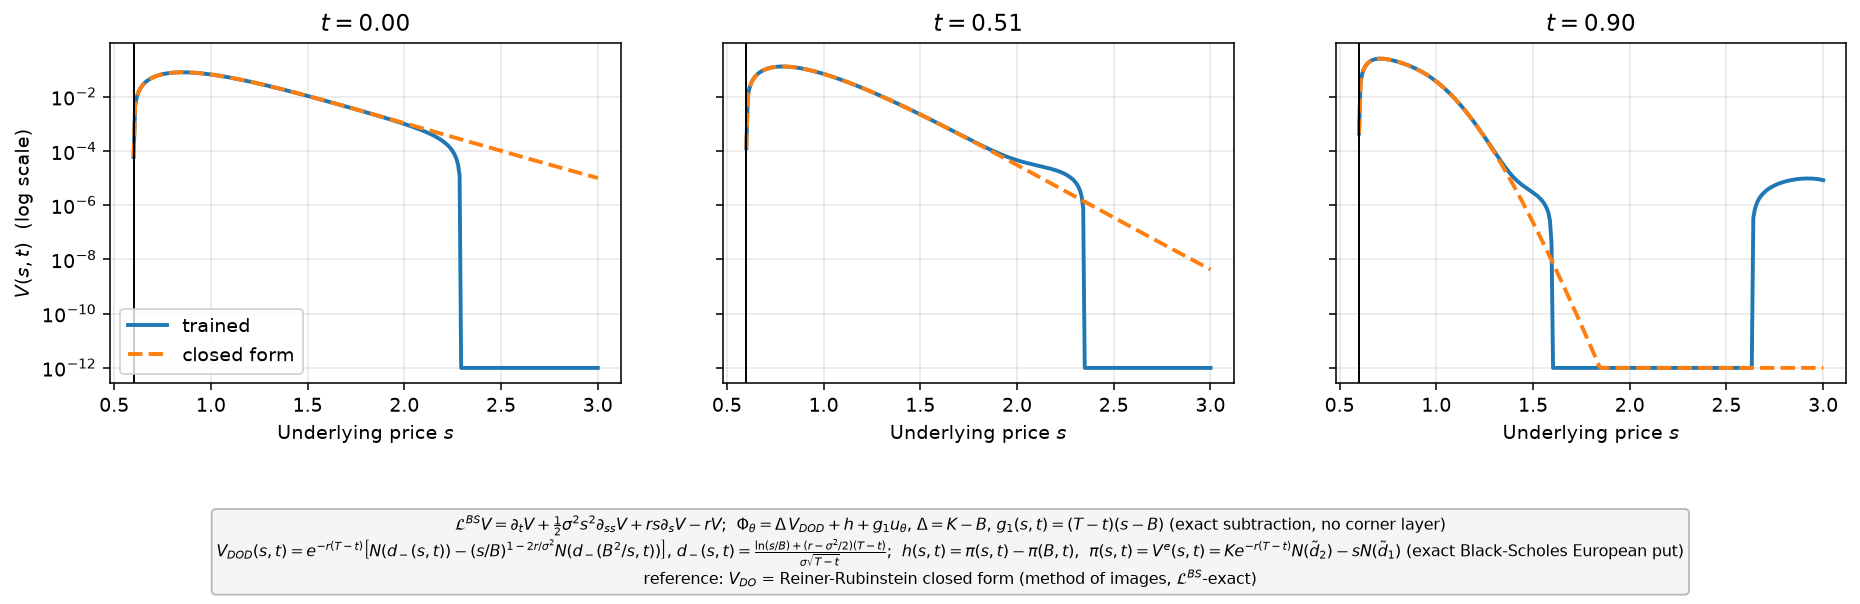
\includegraphics[width=\linewidth]{figures/subtraction_blackscholes_seed0_log_slice_eps0.png}
\caption{Coupes $V(s,t)$ à $t$ fixé, échelle logarithmique (solution entraînée en trait plein, forme fermée en tirets). soustraction exacte ($\Delta V_{DOD}$), profil Black--Scholes $V^e$.}
\label{fig:subtraction_blackscholes-log_slice_eps0}
\end{figure}

\begin{figure}[H]
\centering
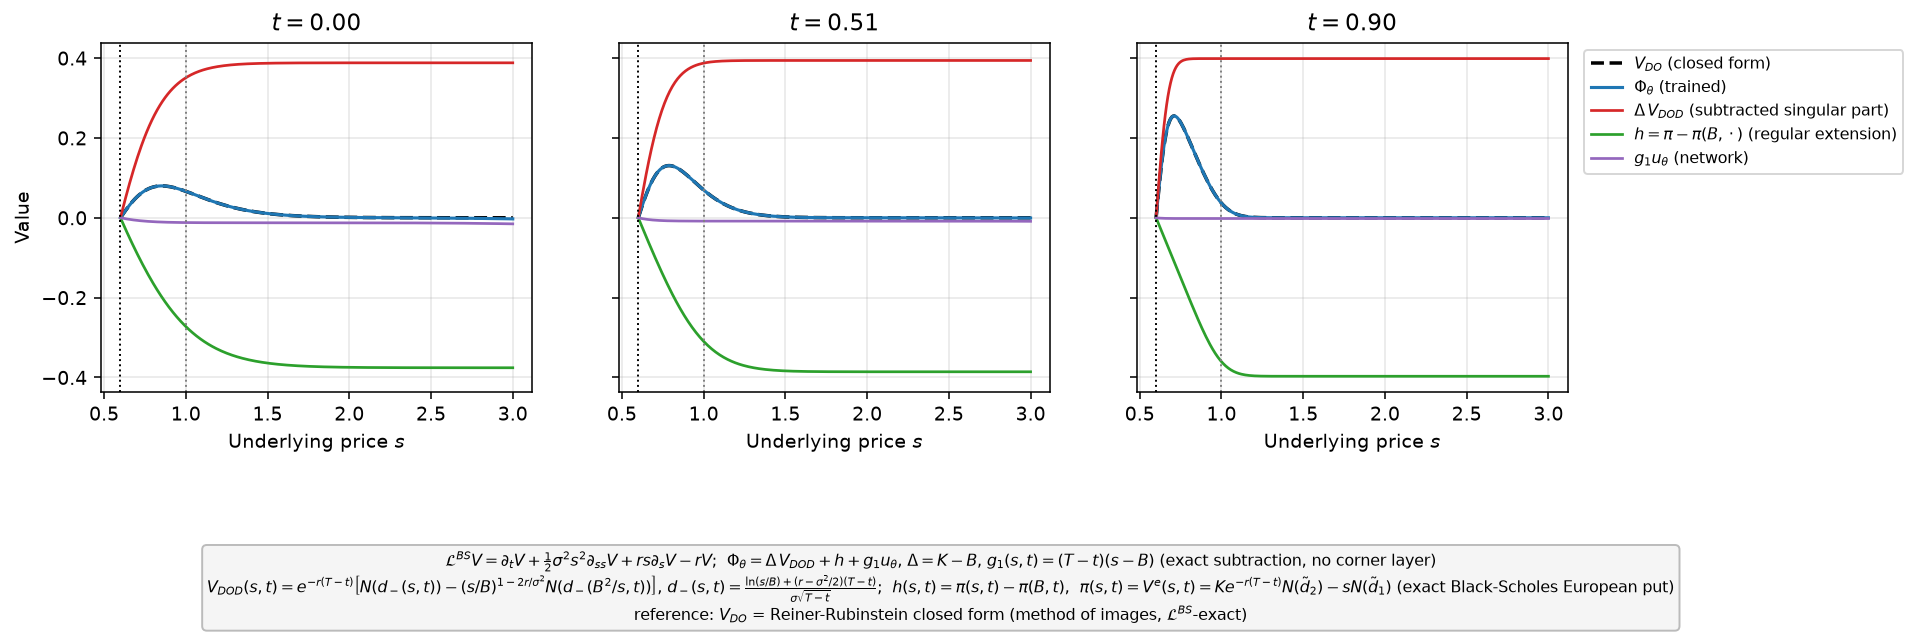
\includegraphics[width=\linewidth]{figures/subtraction_blackscholes_seed0_subtraction_decomposition.png}
\caption{Décomposition de l'estimateur : partie singulière en forme fermée, extension régulière $h$, réseau $g_1u_\theta$, total, contre $V_{DO}$. soustraction exacte ($\Delta V_{DOD}$), profil Black--Scholes $V^e$.}
\label{fig:subtraction_blackscholes-subtraction_decomposition}
\end{figure}

\subsection{Exact subtraction, split-semigroup profile}
soustraction exacte ($\Delta V_{DOD}$), profil split-semigroupe. Run : \path{20260920_210040_iters50000_eps0_seed0_subtraction_split_nuc0.3_closedform}.
\begin{figure}[H]
\centering
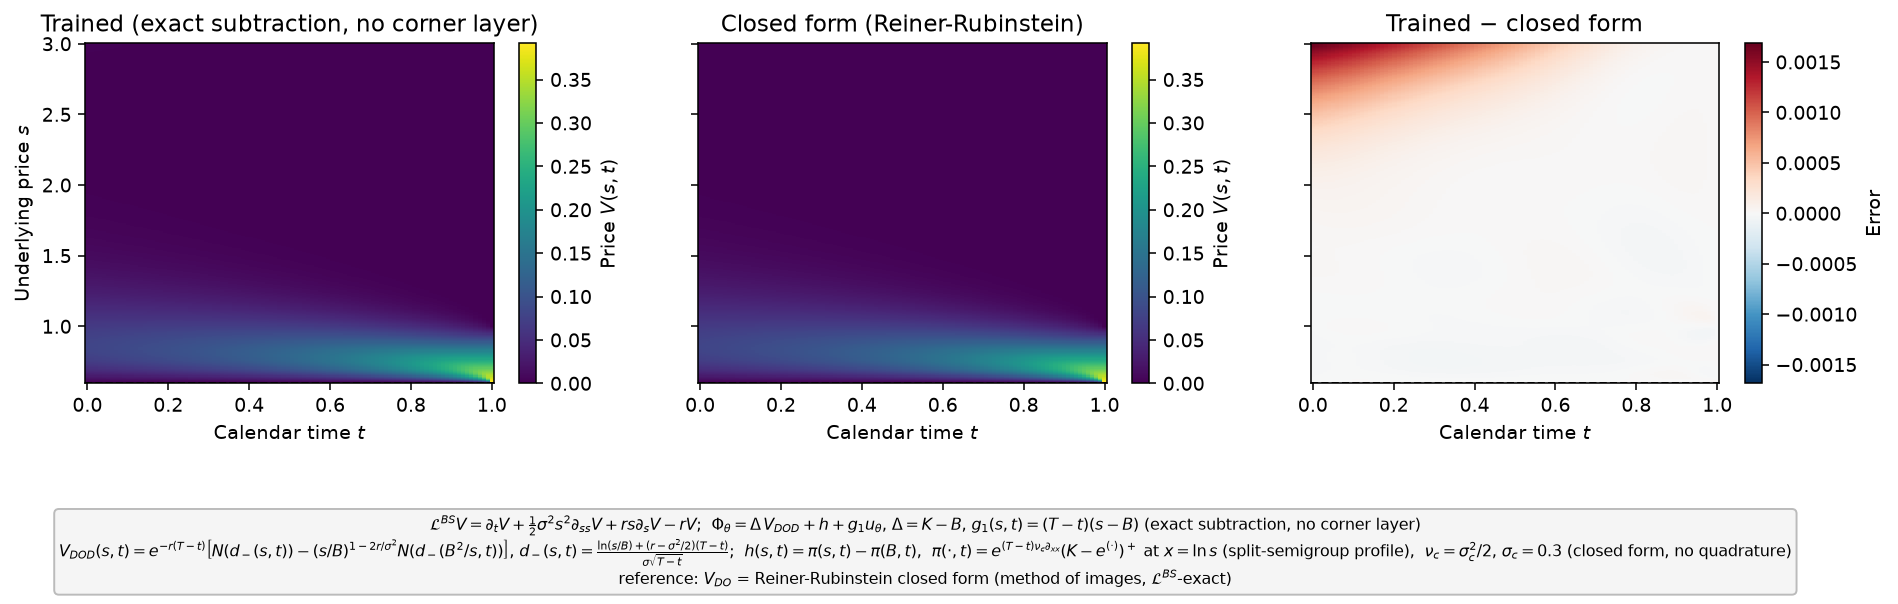
\includegraphics[width=\linewidth]{figures/subtraction_split_seed0_price_surface_eps0.png}
\caption{Surface de prix : solution entraînée, forme fermée, différence. soustraction exacte ($\Delta V_{DOD}$), profil split-semigroupe.}
\label{fig:subtraction_split-price_surface_eps0}
\end{figure}

\begin{figure}[H]
\centering
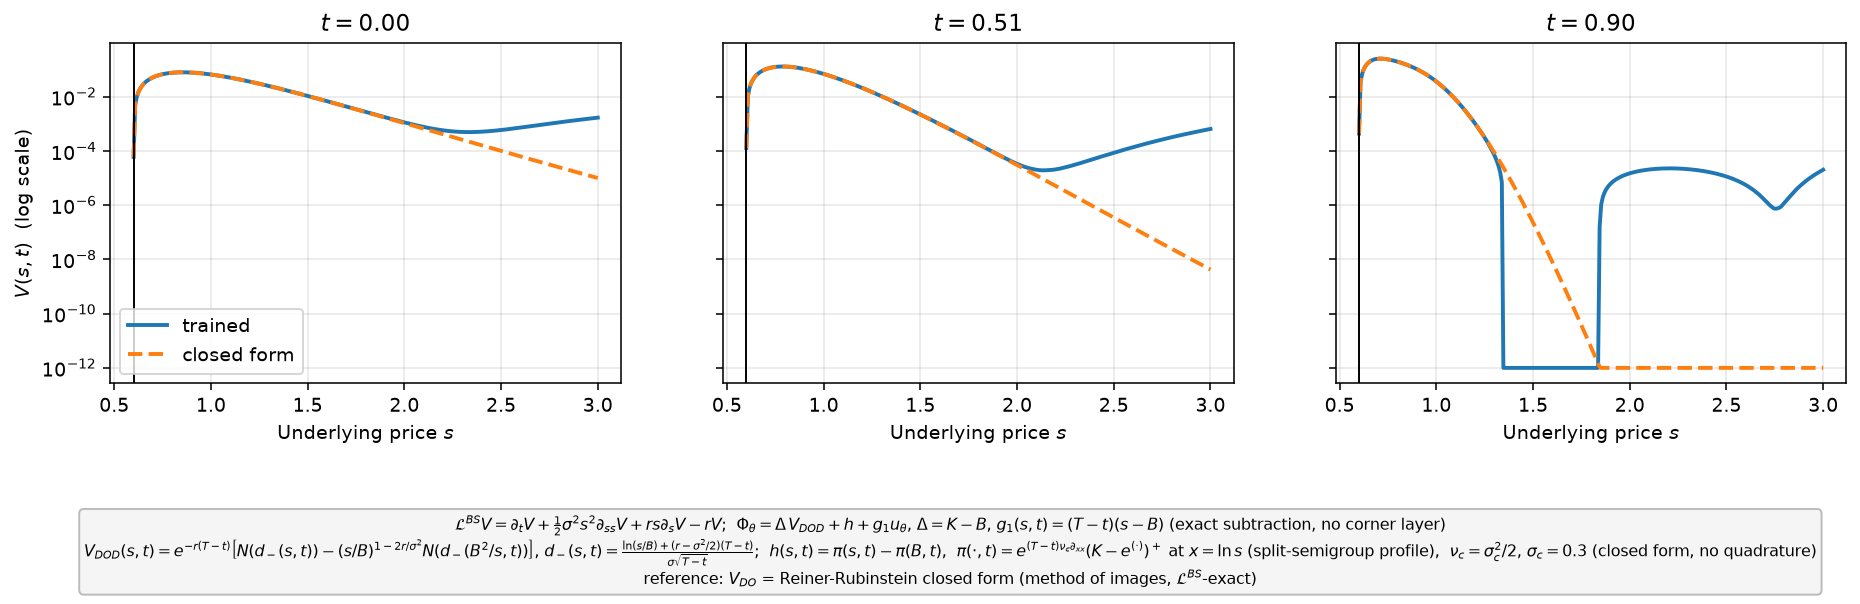
\includegraphics[width=\linewidth]{figures/subtraction_split_seed0_log_slice_eps0.png}
\caption{Coupes $V(s,t)$ à $t$ fixé, échelle logarithmique (solution entraînée en trait plein, forme fermée en tirets). soustraction exacte ($\Delta V_{DOD}$), profil split-semigroupe.}
\label{fig:subtraction_split-log_slice_eps0}
\end{figure}

\begin{figure}[H]
\centering
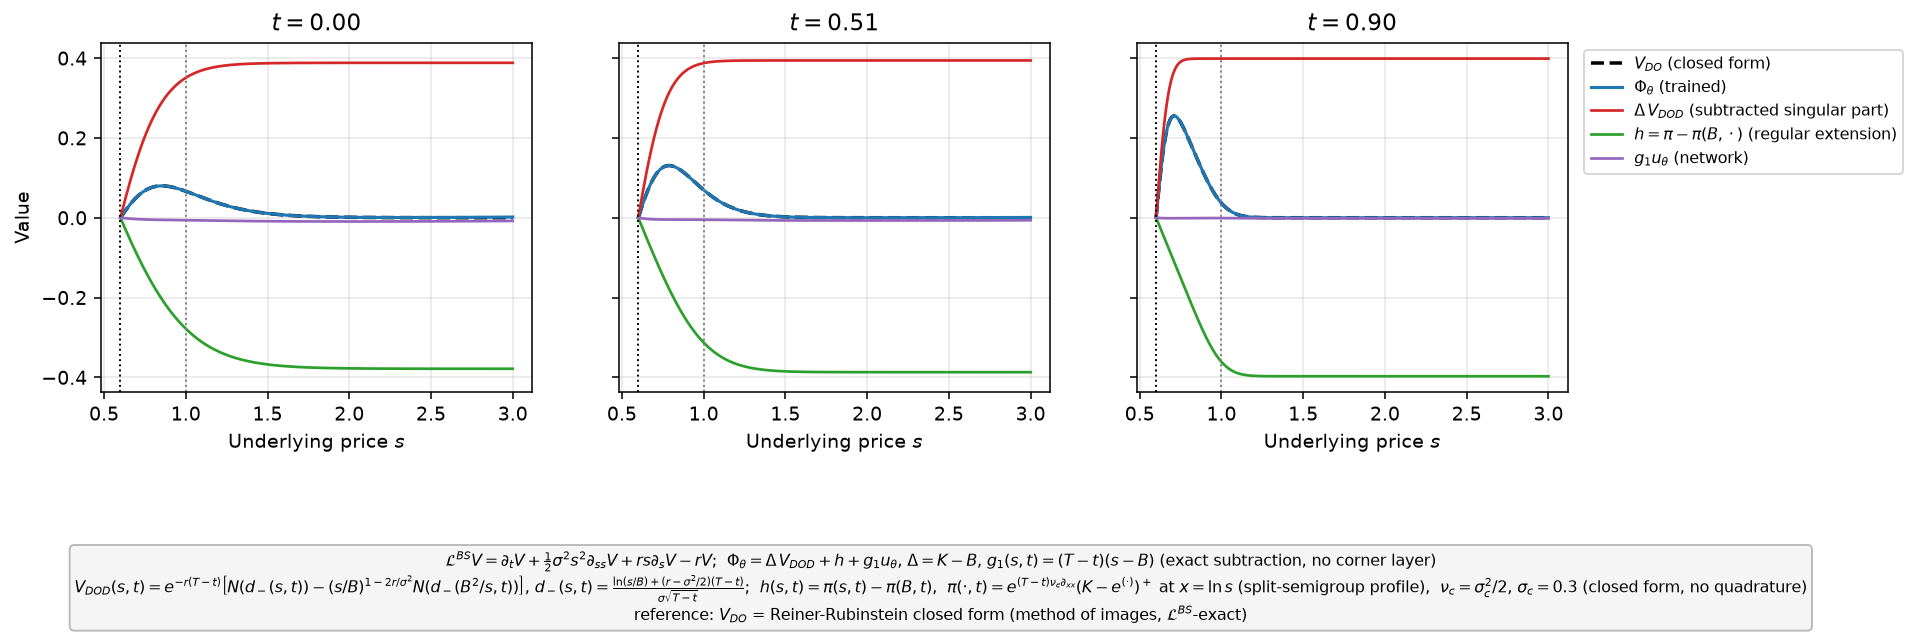
\includegraphics[width=\linewidth]{figures/subtraction_split_seed0_subtraction_decomposition.png}
\caption{Décomposition de l'estimateur : partie singulière en forme fermée, extension régulière $h$, réseau $g_1u_\theta$, total, contre $V_{DO}$. soustraction exacte ($\Delta V_{DOD}$), profil split-semigroupe.}
\label{fig:subtraction_split-subtraction_decomposition}
\end{figure}

\subsection{Corner enrichment, raw payoff profile}
enrichissement du coin ($\chi\Delta\,\mathrm{erf}(\xi)$), profil payoff brut (contrôle négatif). Run : \path{20260921_003020_iters50000_eps0_seed0_enrichment_raw_d00.1_d10.3}.
\begin{figure}[H]
\centering
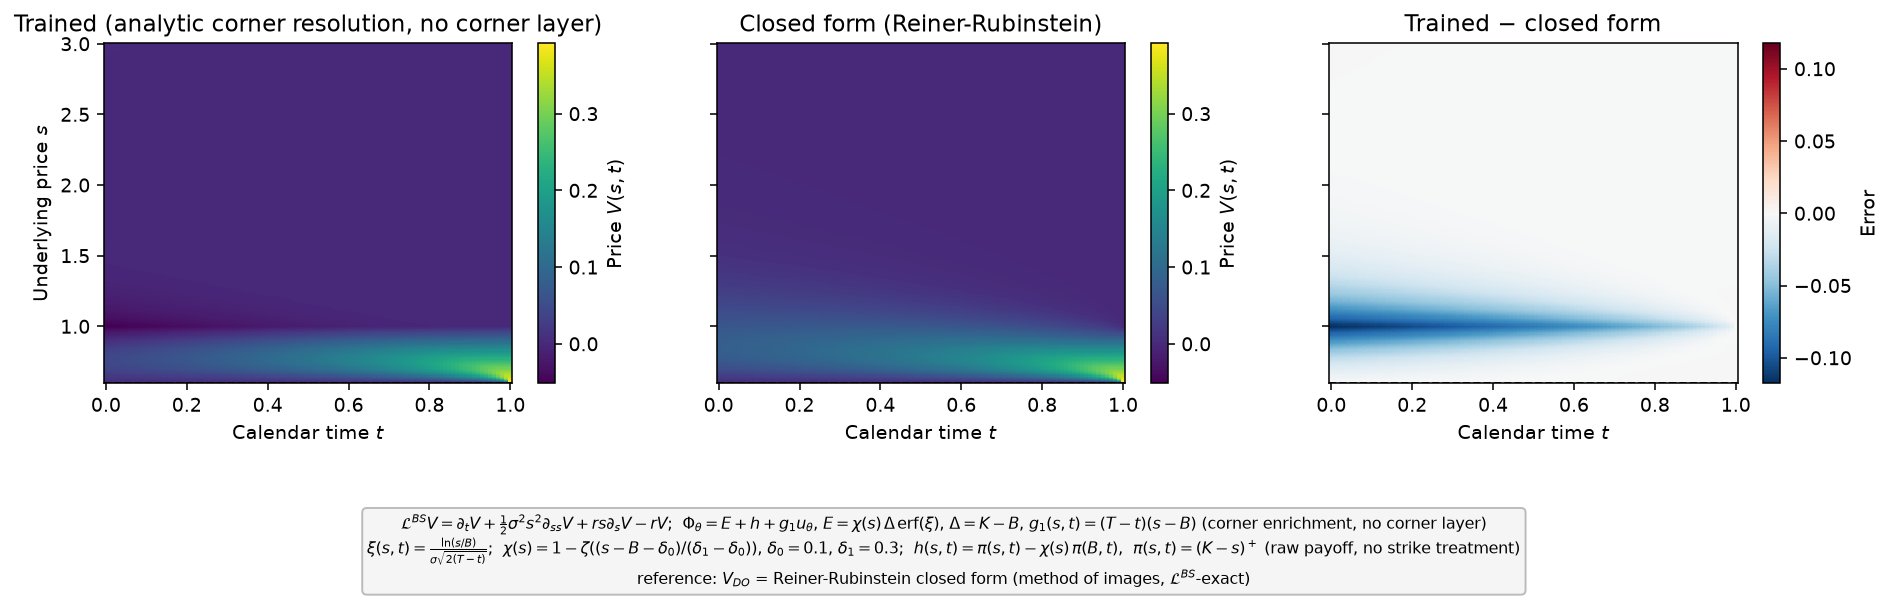
\includegraphics[width=\linewidth]{figures/enrichment_raw_seed0_price_surface_eps0.png}
\caption{Surface de prix : solution entraînée, forme fermée, différence. enrichissement du coin ($\chi\Delta\,\mathrm{erf}(\xi)$), profil payoff brut (contrôle négatif).}
\label{fig:enrichment_raw-price_surface_eps0}
\end{figure}

\begin{figure}[H]
\centering
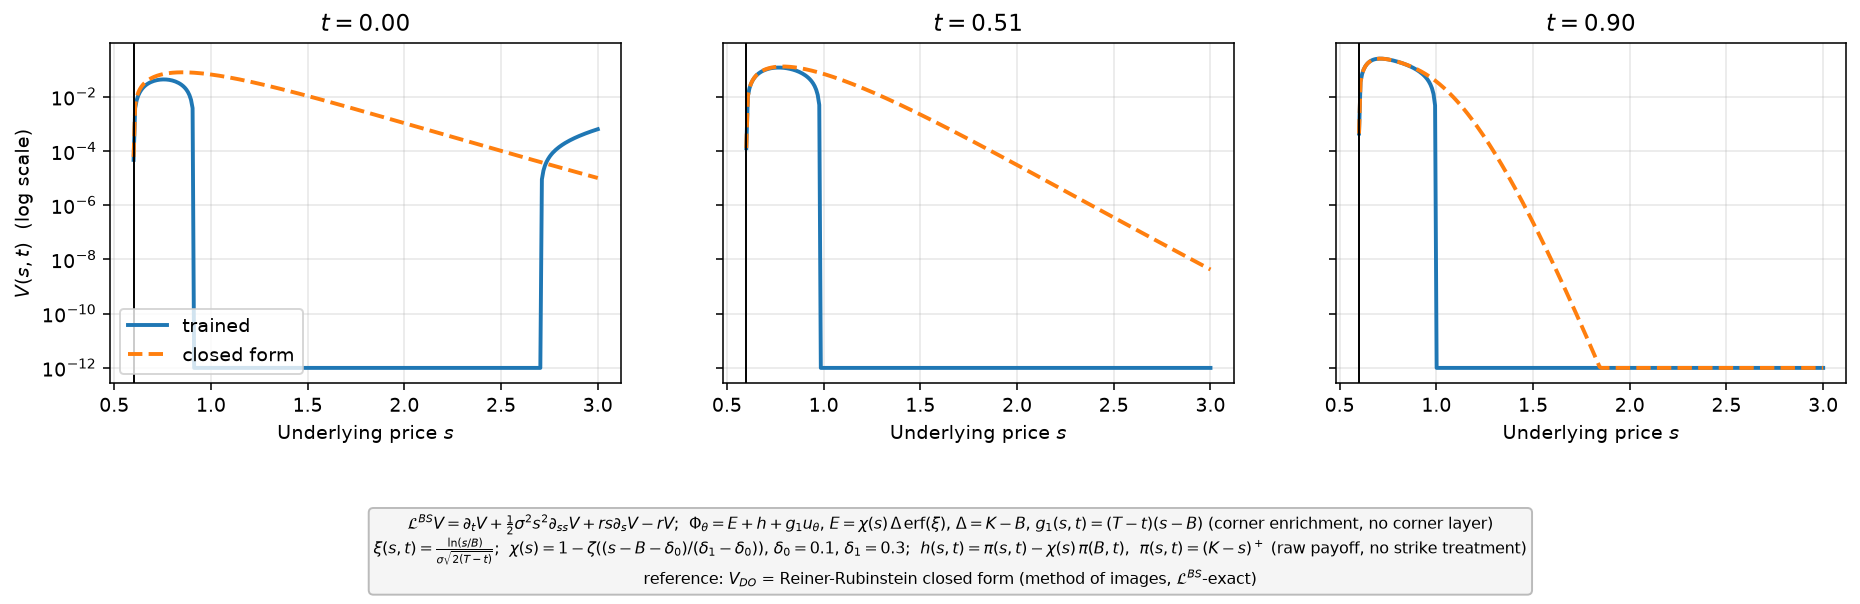
\includegraphics[width=\linewidth]{figures/enrichment_raw_seed0_log_slice_eps0.png}
\caption{Coupes $V(s,t)$ à $t$ fixé, échelle logarithmique (solution entraînée en trait plein, forme fermée en tirets). enrichissement du coin ($\chi\Delta\,\mathrm{erf}(\xi)$), profil payoff brut (contrôle négatif).}
\label{fig:enrichment_raw-log_slice_eps0}
\end{figure}

\begin{figure}[H]
\centering
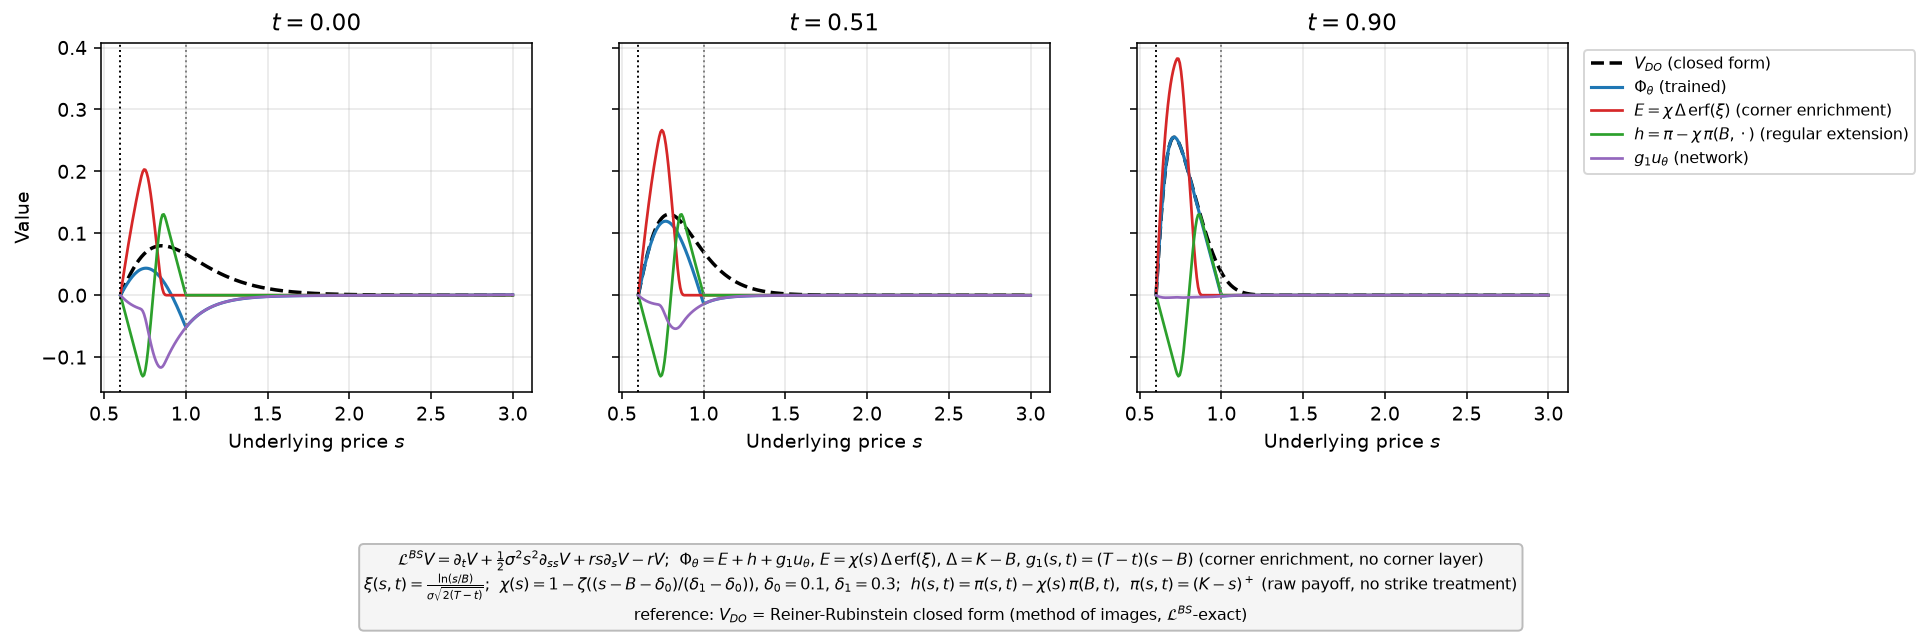
\includegraphics[width=\linewidth]{figures/enrichment_raw_seed0_subtraction_decomposition.png}
\caption{Décomposition de l'estimateur : partie singulière en forme fermée, extension régulière $h$, réseau $g_1u_\theta$, total, contre $V_{DO}$. enrichissement du coin ($\chi\Delta\,\mathrm{erf}(\xi)$), profil payoff brut (contrôle négatif).}
\label{fig:enrichment_raw-subtraction_decomposition}
\end{figure}

\subsection{Corner enrichment, Black-Scholes profile}
enrichissement du coin ($\chi\Delta\,\mathrm{erf}(\xi)$), profil Black--Scholes $V^e$. Run : \path{20260921_003313_iters50000_eps0_seed0_enrichment_blackscholes_d00.1_d10.3}.
\begin{figure}[H]
\centering
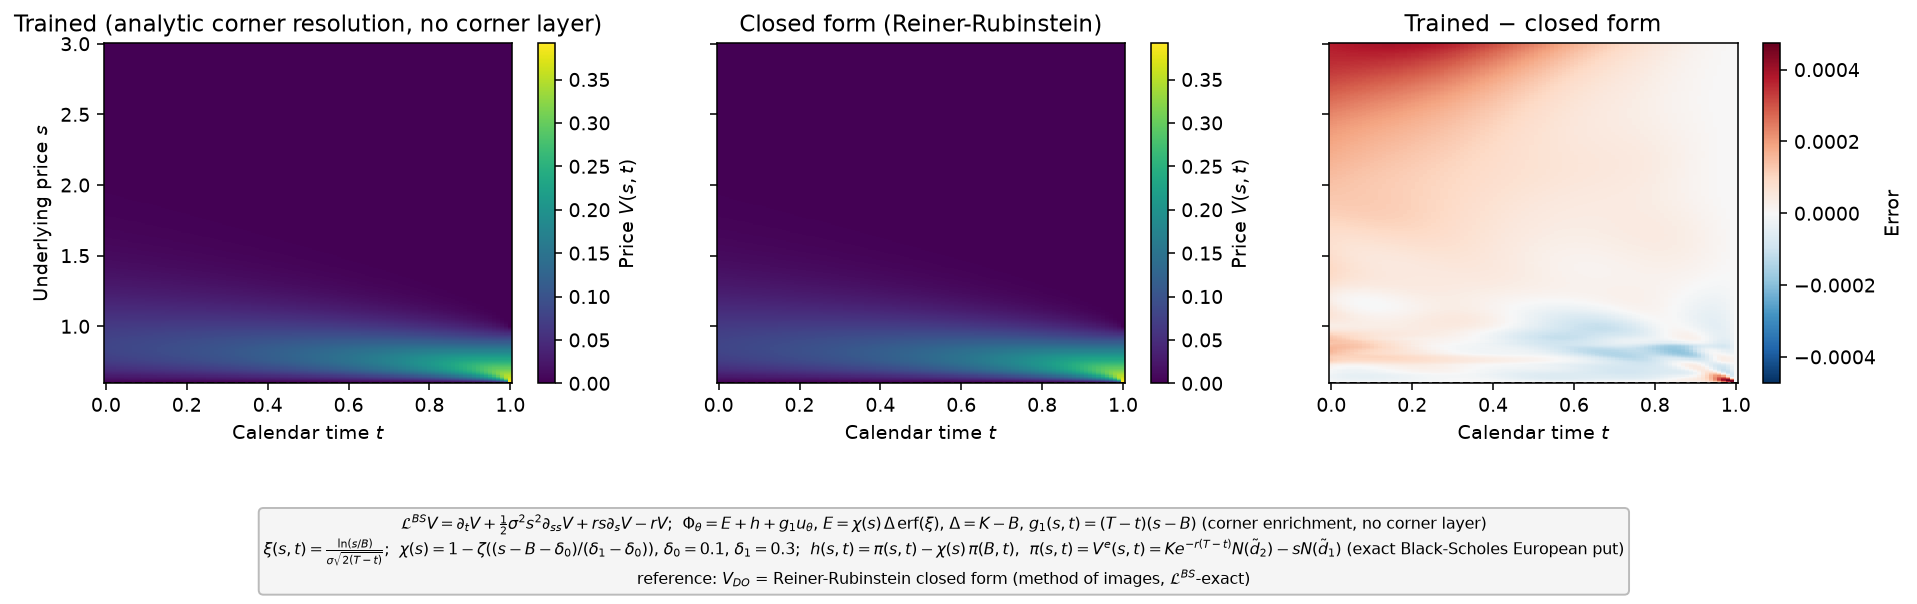
\includegraphics[width=\linewidth]{figures/enrichment_blackscholes_seed0_price_surface_eps0.png}
\caption{Surface de prix : solution entraînée, forme fermée, différence. enrichissement du coin ($\chi\Delta\,\mathrm{erf}(\xi)$), profil Black--Scholes $V^e$.}
\label{fig:enrichment_blackscholes-price_surface_eps0}
\end{figure}

\begin{figure}[H]
\centering
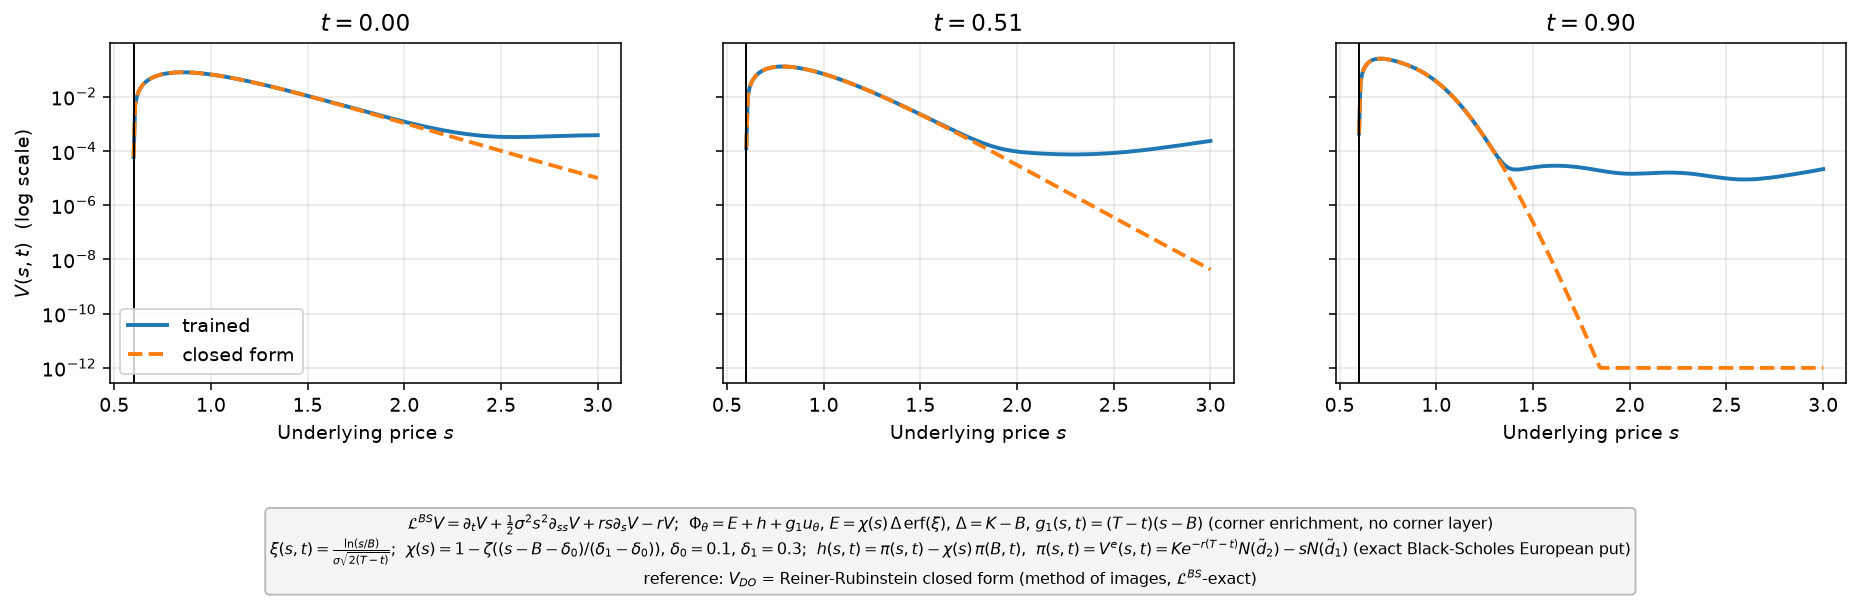
\includegraphics[width=\linewidth]{figures/enrichment_blackscholes_seed0_log_slice_eps0.png}
\caption{Coupes $V(s,t)$ à $t$ fixé, échelle logarithmique (solution entraînée en trait plein, forme fermée en tirets). enrichissement du coin ($\chi\Delta\,\mathrm{erf}(\xi)$), profil Black--Scholes $V^e$.}
\label{fig:enrichment_blackscholes-log_slice_eps0}
\end{figure}

\begin{figure}[H]
\centering
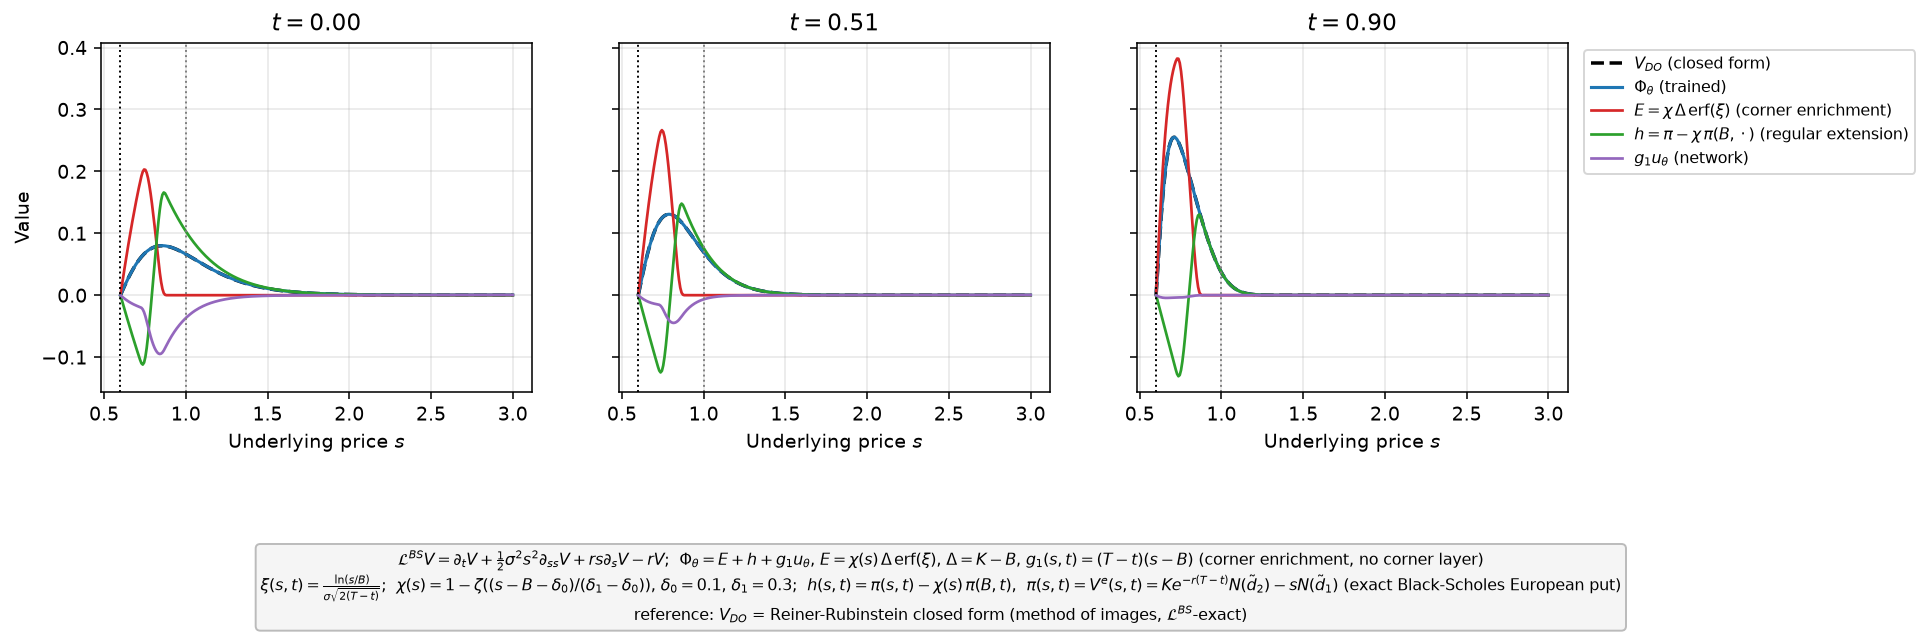
\includegraphics[width=\linewidth]{figures/enrichment_blackscholes_seed0_subtraction_decomposition.png}
\caption{Décomposition de l'estimateur : partie singulière en forme fermée, extension régulière $h$, réseau $g_1u_\theta$, total, contre $V_{DO}$. enrichissement du coin ($\chi\Delta\,\mathrm{erf}(\xi)$), profil Black--Scholes $V^e$.}
\label{fig:enrichment_blackscholes-subtraction_decomposition}
\end{figure}

\subsection{Corner enrichment, split-semigroup profile}
enrichissement du coin ($\chi\Delta\,\mathrm{erf}(\xi)$), profil split-semigroupe. Run : \path{20260921_011735_iters50000_eps0_seed0_enrichment_split_d00.1_d10.3_nuc0.3_closedform}.
\begin{figure}[H]
\centering
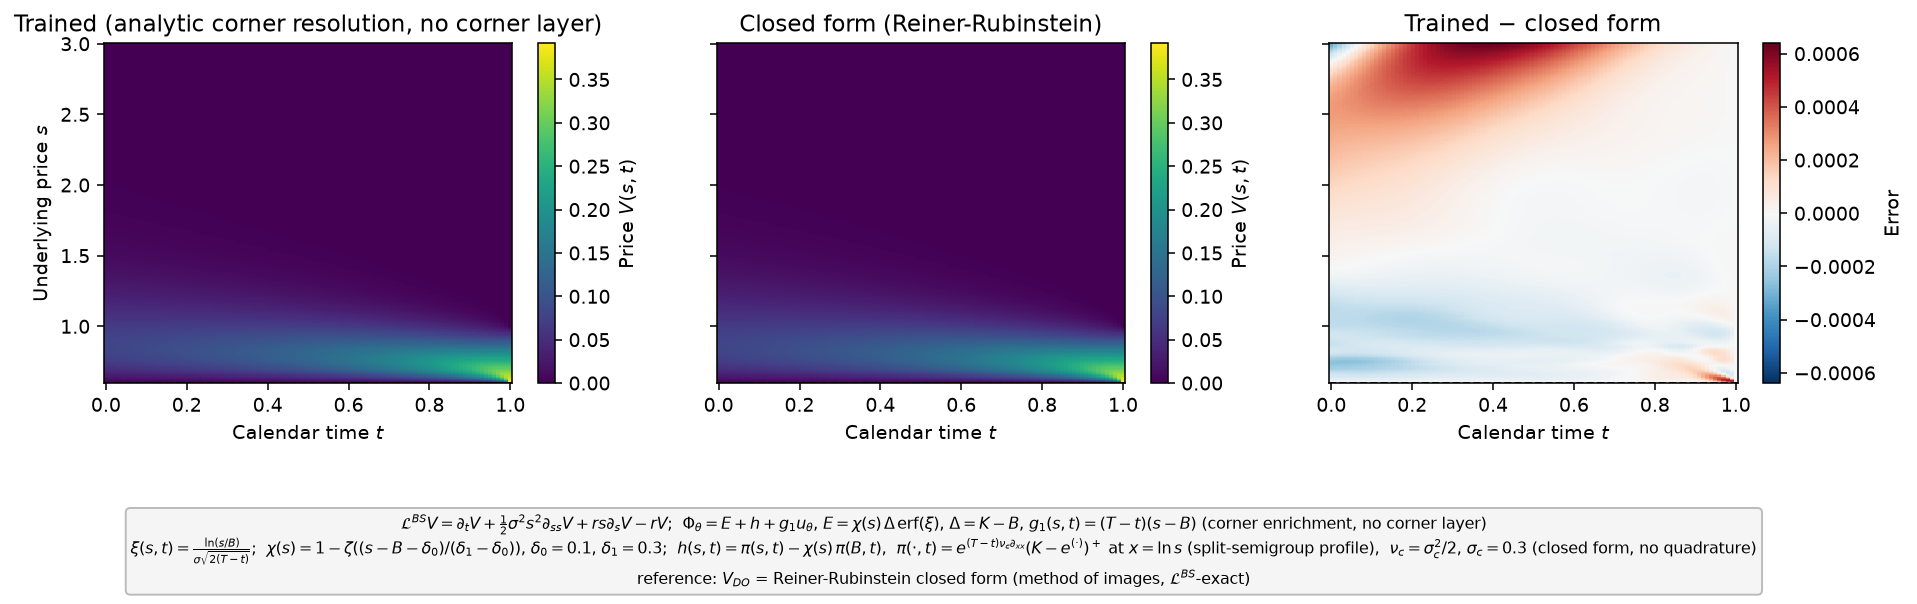
\includegraphics[width=\linewidth]{figures/enrichment_split_seed0_price_surface_eps0.png}
\caption{Surface de prix : solution entraînée, forme fermée, différence. enrichissement du coin ($\chi\Delta\,\mathrm{erf}(\xi)$), profil split-semigroupe.}
\label{fig:enrichment_split-price_surface_eps0}
\end{figure}

\begin{figure}[H]
\centering
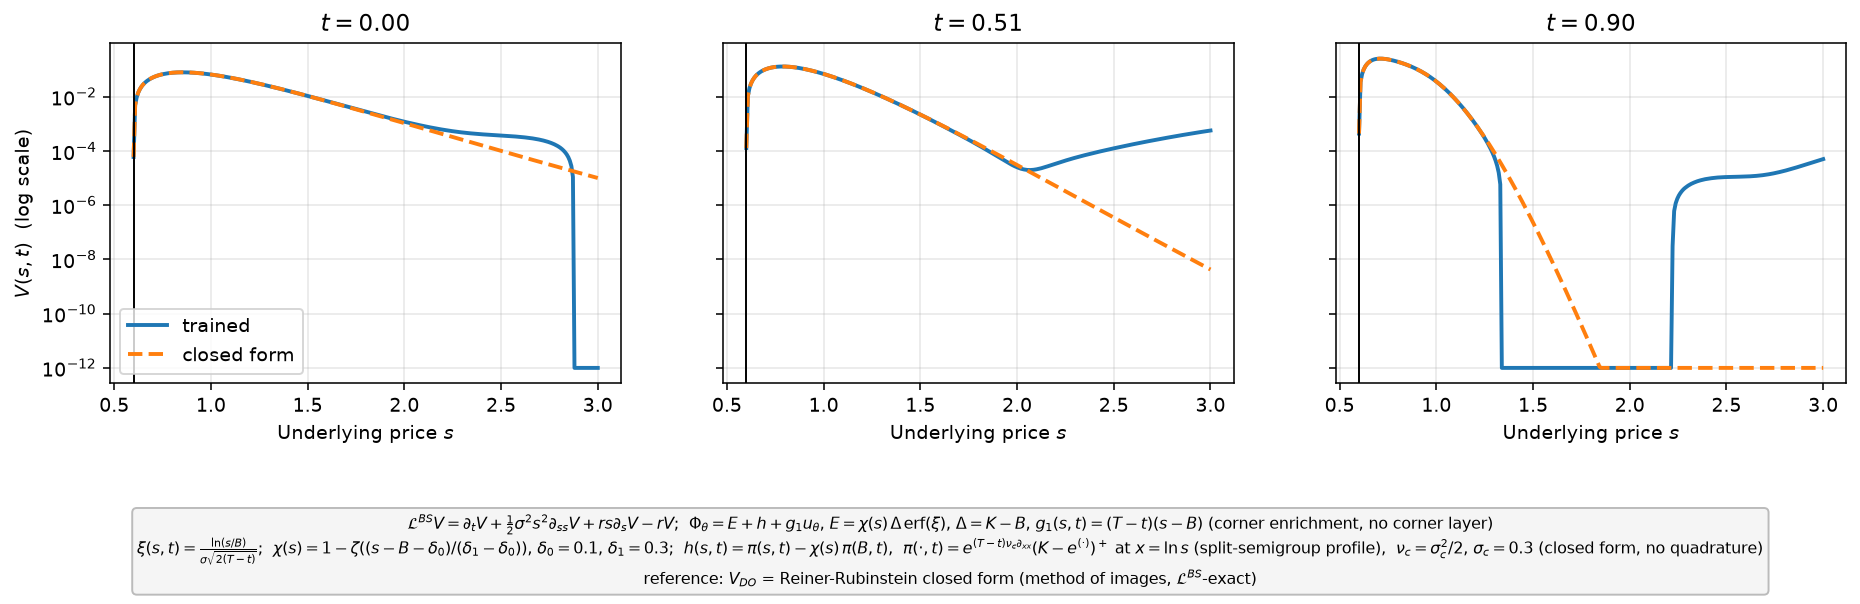
\includegraphics[width=\linewidth]{figures/enrichment_split_seed0_log_slice_eps0.png}
\caption{Coupes $V(s,t)$ à $t$ fixé, échelle logarithmique (solution entraînée en trait plein, forme fermée en tirets). enrichissement du coin ($\chi\Delta\,\mathrm{erf}(\xi)$), profil split-semigroupe.}
\label{fig:enrichment_split-log_slice_eps0}
\end{figure}

\begin{figure}[H]
\centering
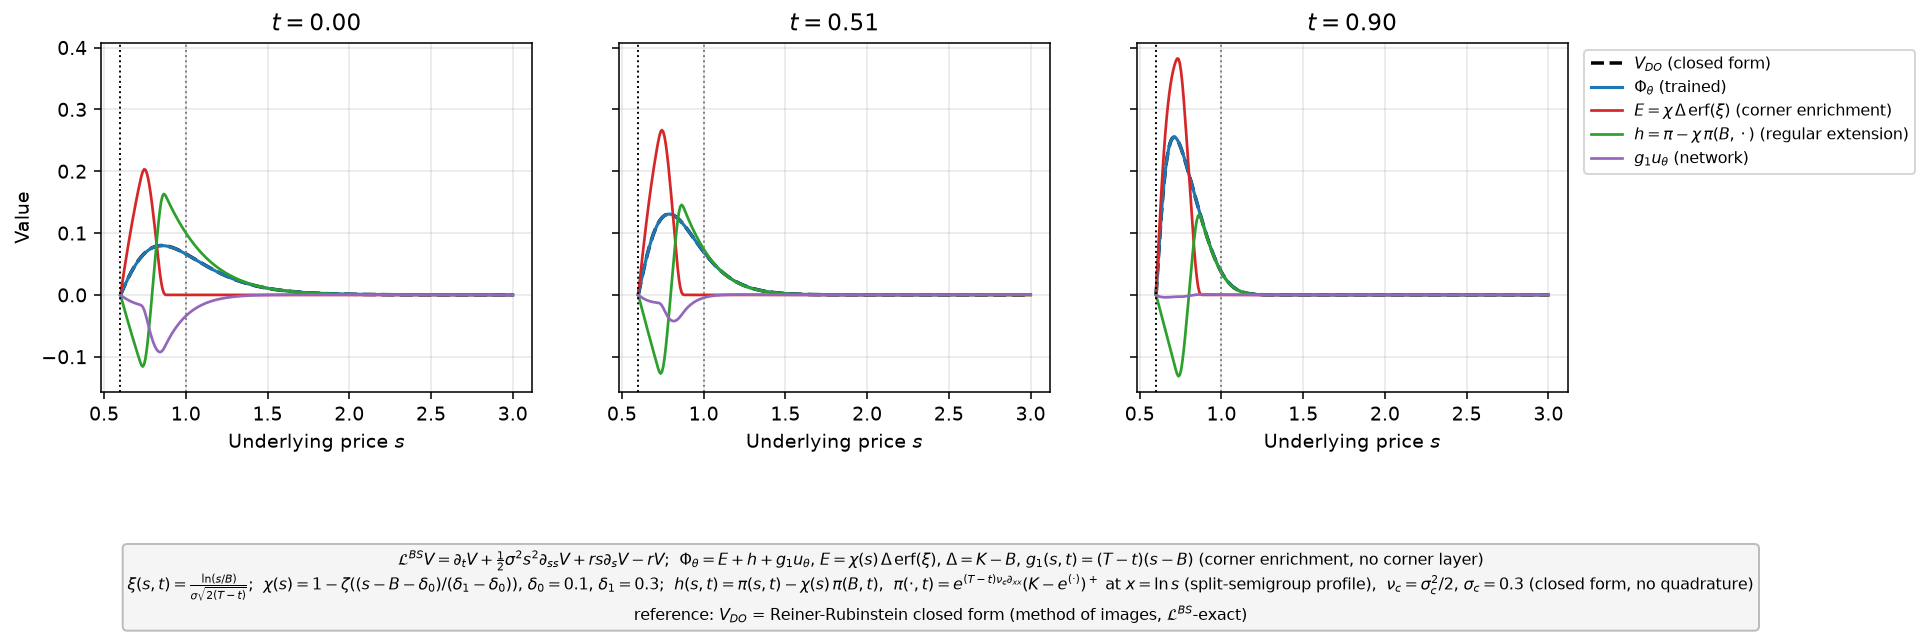
\includegraphics[width=\linewidth]{figures/enrichment_split_seed0_subtraction_decomposition.png}
\caption{Décomposition de l'estimateur : partie singulière en forme fermée, extension régulière $h$, réseau $g_1u_\theta$, total, contre $V_{DO}$. enrichissement du coin ($\chi\Delta\,\mathrm{erf}(\xi)$), profil split-semigroupe.}
\label{fig:enrichment_split-subtraction_decomposition}
\end{figure}

\end{document}
